% Emacs settings: -*-mode: latex; TeX-master: "manual.tex"; -*-

\chapter{Running \MCS}
\label{c:running}

This chapter describes usage of the \MCS simulation package. 
In case of problems regarding installation or usage, the \MCS mailing
list~\cite{mcstas_webpage} or the authors should be contacted.

\index{McStas!structure}
Performing a simulation using \MCS can be divided into the following
steps/elements
\begin{itemize}
\item{The structure of \MCS is illustrated in
    Figure~\ref{fig:structure}.}
\item{To use \MCS, an instrument
definition file describing the instrument to be simulated must be
written. Alternatively, an example instrument file can be obtained
from the \verb+examples/+ directory in the distribution or from
another source.}
\item{The input files (instrument and component files) are written in the \MCS
meta-language and are edited either by using your favorite editor
or by using the built-in editor of the graphical user interface
(\texttt{mcgui}).}
\item{Next, the \MCS compiler \mcs is invoked to translate the instrument and component files into a C program. The program \mcs itself is written in C, using the parser \textit{flex} and the compiler compiler \textit{bison}.}
\item{The resulting C program can then be
compiled with a C compiler and run in combination with various
front-end programs for example to present the intensity at the
detector as a motor position is varied.}
\item{The output data may be analyzed and visualized in the same way as regular
    experiments by using the data handling and visualization tools in \MCS.
    As of \MCS 3.x, these front-ends (\texttt{mcplot}, \texttt{mcdisplay},
    \texttt{mcresplot}, \ldots) are all implemented in Python, using
    \texttt{matplotlib}, \texttt{pyqtgraph} and browser/HTML (D3.js) back-ends,
    see section~\ref{s:frontends}. Further data output formats including NeXus
    are available, see section \ref{s:analyze}.\index{Tools}}
\end{itemize}


\begin{figure}[pt!]
\begin{center}
    \includegraphics[width=\textwidth]{figures/mcstas_software.pdf}
\end{center}
\caption{An illustration of the structure of \MCS.\index{McStas!structure}}
\label{fig:structure}
\end{figure}

%%%%%%%%%%%%%%%%%%%%%%%%%%%%%%%%%%%%%%%%%%%%%%%%%%%%%%%%%%%%%%%%%%%%%%%%%%%%%%%%
\section{Installation and updates}
\label{s:install}

\index{McStas!installation}
\index{Installation}
For installation notes, see the web site~\cite{mcstas_webpage}.
In case of problems, write the support mailing list,
or contact the authors.

% -------------------------------------------------------------------------------
\subsubsection{Installation via conda-forge (recommended)}
\label{s:install-conda}

The recommended installation method for all supported platforms---Linux,
macOS, and Windows---is via the \texttt{conda-forge} channel.  Once a
conda-compatible environment manager such as Miniforge or Mambaforge is
available, \MCS can be installed into a fresh conda environment:

\begin{verbatim}
  conda create -n mcstas -c conda-forge mcstas
  conda activate mcstas
  mcgui
\end{verbatim}

On Windows a dedicated \texttt{mcstas-conda} batch script is provided by
the installer.  After it completes, use the \emph{mcstas-shell} desktop
shortcut and issue \texttt{mcgui} to start the graphical interface.
Arm64 Windows is also supported via this route.

For full platform-specific installation instructions, including Linux
package management and macOS options, see:
\begin{center}
  \url{https://github.com/mccode-dev/McCode/tree/main/INSTALL-McStas}
\end{center}

\subsection{Important note for Windows users} 
\index{Windows!file and directory names with spaces}
It is a known problem that some of
the \MCS tools do not support filenames / directories with spaces.
We recommend avoiding spaces in the paths used for \MCS work directories
and instrument files. As of \MCS 3.x, all tools (\texttt{mcgui}, \texttt{mcrun},
\texttt{mcplot}, \texttt{mcdisplay}, \ldots) are pure Python and are bundled
with the \texttt{conda-forge} package, so no separate Perl installation is
required on any platform, including Windows.

%-------------------------------------------------------------------------------
\subsection{New releases of \MCS}
\index{McStas!release scheme}
\index{Release scheme}

Releases of new versions of a software package can today be carried out more or
less continuously. However, users do not update their software on a daily basis,
and as a compromise we have adopted the following policy of \MCS .

\begin{itemize}
\item The versions {\version}.x will possibly contain bug fixes and minor new
  functionality. A new manual will, however, not be released and the
  modifications are documented on the \MCS web-page. The extensions of the
  forthcoming version {\version}.x are also listed on the web, and new versions
  may be released quite frequently when it is requested by the user community.
\end{itemize}


%%%%%%%%%%%%%%%%%%%%%%%%%%%%%%%%%%%%%%%%%%%%%%%%%%%%%%%%%%%%%%%%%%%%%%%%%%%%%%%%
\section{Brief introduction to the graphical user interface}
\label{s:brief}

\index{McStas!running from the GUI|(}
\indexMCTOOL{mcgui}{(textbf}

This section gives an ultra-brief overview of how to use \MCS once it
has been properly installed. It is intended for those who do not read
manuals if they can avoid it. For details on the different steps, see
the following sections. This section uses the
\verb+BNL_H8.instr+ file supplied in the \verb+examples/BNL/BNL_H8+
directory of the \MCS distribution.

To start the graphical user interface of \MCS, run the
\verb+mcgui+ command which will open a window
with a number of menus,
see figure~\ref{fig:mcgui}. 
\begin{figure}[htb!]
  \begin{center}
    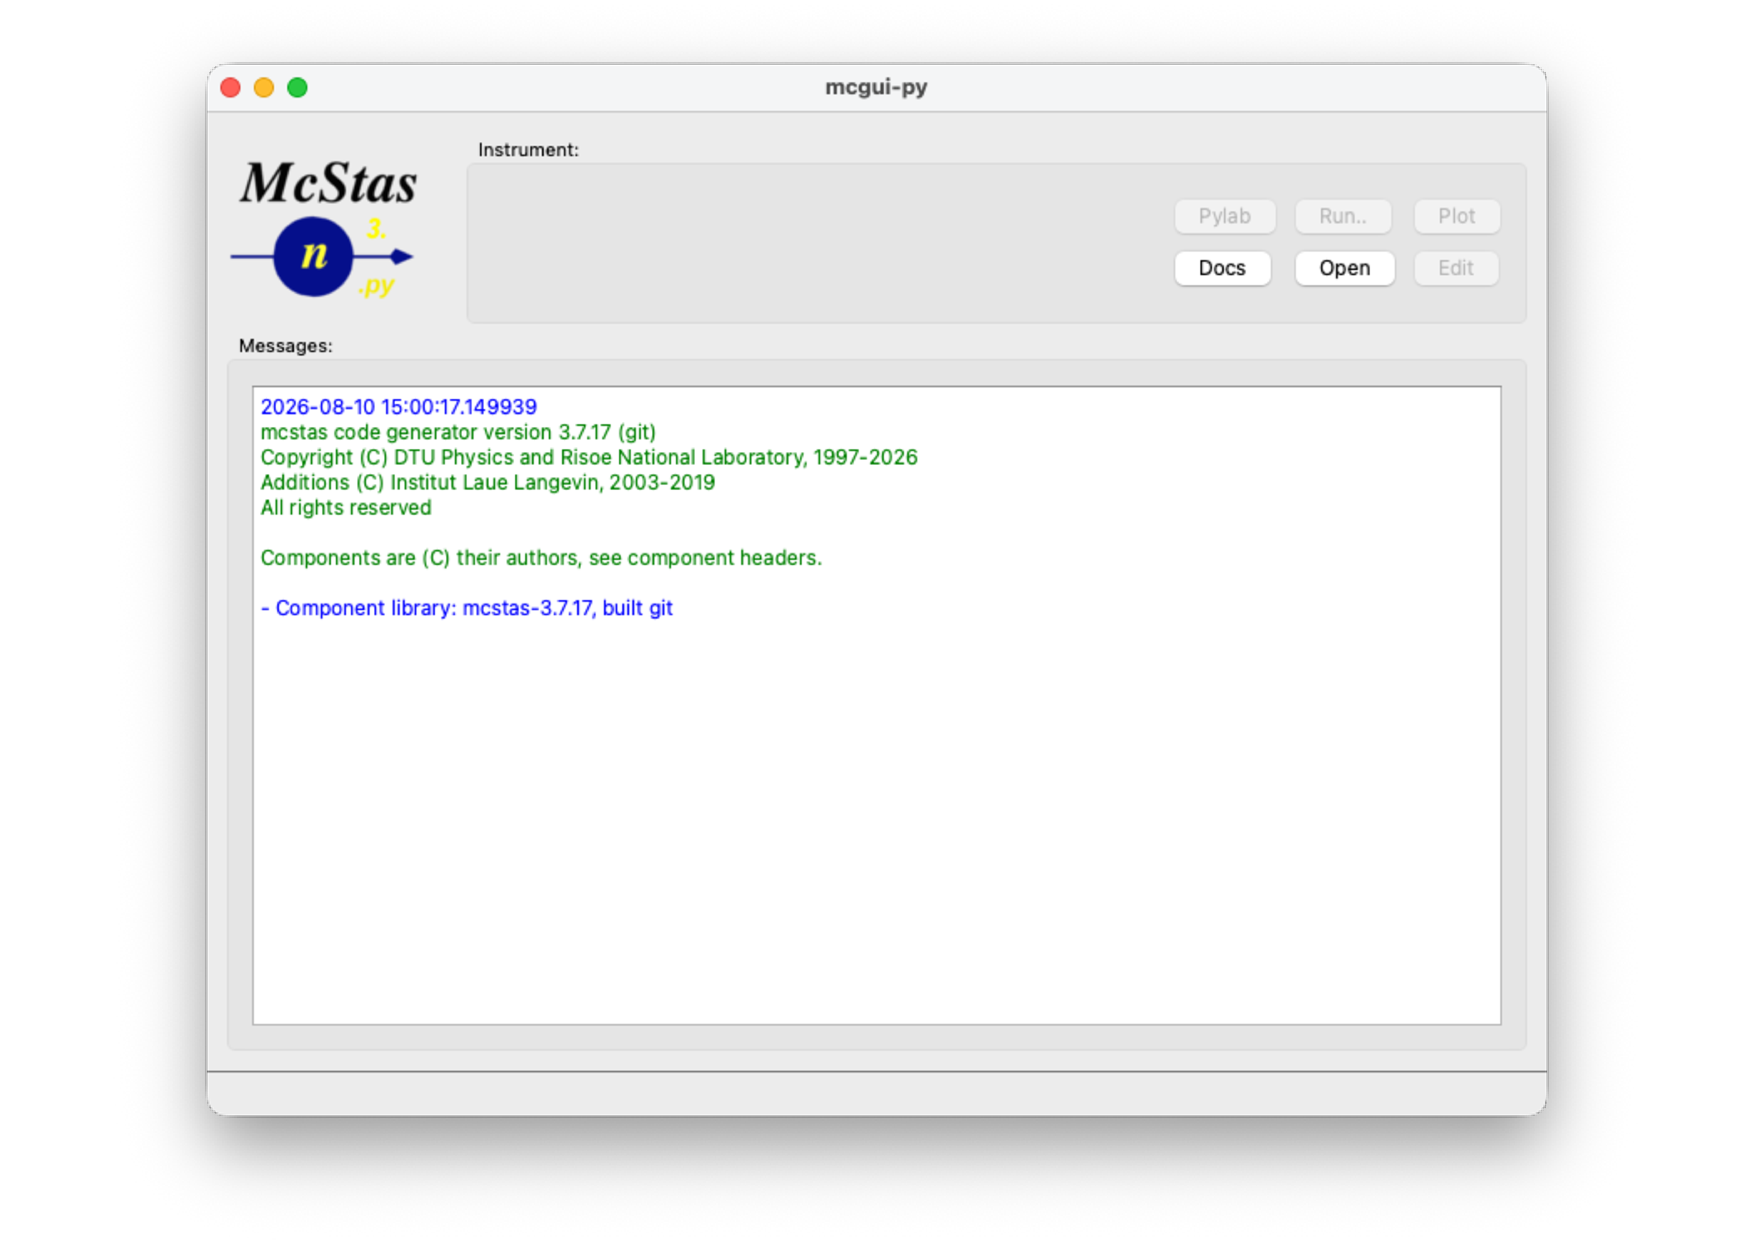
\includegraphics[width=0.75\textwidth]{figures/mcgui}
  \end{center}
\caption{The graphical user interface \texttt{mcgui}.}
\label{fig:mcgui}
\end{figure}
\label{p:neutronsite}
To load an instrument, select ``New from Template'' (formerly known as the
``Neutron site'' menu) and open the template/example \verb+BNL/BNL_H8+.
Next, check that the current plotting backend setting (``Preferences'' in the
\textbf{File} menu, or the \verb+--autoplotter+ option of \verb+mcrun+)
corresponds to your system setup:
\begin{itemize}
\item{by editing the user configuration file, see \verb+mcrun --edit-user-config+,}
\end{itemize}
\indexEV{MCSTAS\_FORMAT}

Next, select ``Run simulation'' from the ``Simulation'' menu.
The \MCS compiler \mcs will translate the definition into an executable program.
Then \texttt{mcgui} will pop up a dialog window.
Type a value for the ``ROT'' parameter ({\em e.g.}
90), check the ``Plot results'' option, and select ``Start''. The
simulation will run, and when it finishes after a while the results will
be plotted in a window, using one of the Python plotting back-ends
(\texttt{matplotlib}, \texttt{pyqtgraph} or an HTML/browser view), see
section~\ref{s:mcplot}.\indexMCTOOL{mcplot}{} For other options, execute
\verb+mcplot --help+ to get help.

To visualize or
debug the simulation graphically, repeat the steps but check the ``Trace''
option instead of the ``Simulate'' option.  A window will pop up showing a
sketch of the instrument, drawn by the \texttt{mcdisplay} front-end
(section~\ref{s:mcdisplay}), again using one of the \texttt{matplotlib},
\texttt{pyqtgraph} or webGL back-ends.

For a slightly longer gentle introduction to \MCS, see the \MCS tutorial
(available from~\cite{mcstas_webpage}), and as of version \version\ built into
the \verb+mcgui+ help menu. For more technical details, read on from
section~\ref{s:running}

\indexMCTOOL{mcgui}{)}
\index{McStas!running from the GUI|)}


%%%%%%%%%%%%%%%%%%%%%%%%%%%%%%%%%%%%%%%%%%%%%%%%%%%%%%%%%%%%%%%%%%%%%%%%%%%%%%%%
\section{Running the instrument compiler}
\label{s:running}

\indexMCSW{mcstas}{compiler}{(textbf}
This section describes how to run the \MCS compiler \mcs\ manually. Often,
it will be more convenient to use the front-end program \verb+mcgui+
(section~\ref{s:mcgui}) or \verb+mcrun+ (section~\ref{s:mcrun}),
which run the compilation and the simulations automatically.

Upon a command of the form
\begin{bash}
    mcstas name.instr
\end{bash}
the compiler \mcs will read the instrument definition \verb+name.instr+,
written in the \MCS meta-language,
and translate it into a Monte Carlo simulation program in
the programming language C.
The output is by default written to a file in the current
directory with the same name as the instrument file, but with extension
\verb+.c+ rather than \verb+.instr+. This can be overridden using the
\verb+-o+ option as follows:
\begin{bash}
    mcstas -o code.c name.instr
\end{bash}
which gives the output in the file \verb+code.c+.
A single dash `\verb+-+' may be used for both input and output filename
to represent standard input and standard output, respectively.


%-------------------------------------------------------------------------------
\subsection{Code generation options}
\index{Code generation!options}

By default, the code generated by \mcs is ISO-C with
some extensions (currently the only extension is the creation of new
directories, which is not possible in pure ISO-C). The use of
extensions may be disabled with the \verb+-p+ or \verb+--portable+
option. With this option, the output is strictly ISO-C compliant, at
the cost of some slight reduction in capabilities.

The \verb+-t+ or \verb+--trace+ option puts special ``trace'' code in
the output. This code makes it possible to get a complete trace of the
path of every neutron ray through the instrument, as well as the position
and orientation of every component. This option is mainly used with the
\verb+mcdisplay+ front-end as described in section~\ref{s:mcdisplay}.

The code generation options can also be controlled by using preprocessor
macros in the C compiler, without the need to re-run \mcs.
If the preprocessor macro \verb+MC_PORTABLE+ is defined, the
same result is obtained as with the \verb+--portable+ option.
The effect of the \verb+--trace+ option may be obtained
by defining the \verb+MC_TRACE_ENABLED+ macro. Most Unix-like C
compilers allow preprocessor macros to be defined using the \verb+-D+
option, e.g.
\begin{bash}
    cc -DMC_TRACE_ENABLED -DMC_PORTABLE ...
\end{bash}
Finally, the \verb+--verbose+ option will list the components and libraries being
included in the instrument.

\subsubsection{Alternative code generator: \texttt{mccode-antlr}}
\label{s:antlr}

From \MCS~3.5 onwards an alternative code generator,
\texttt{mcstas-antlr}, is available alongside the classic generator.
It is built on the ANTLR parser framework rather than the traditional
\texttt{lex}/\texttt{yacc} toolchain, is implemented primarily in Python,
and is a candidate replacement for the default generator in future releases.

Select it on a per-run basis with the \texttt{--cogen} flag:
\begin{verbatim}
  mcrun --cogen=mcstas-antlr MyInstrument.instr -n 1e8
\end{verbatim}

The active code generator can also be set permanently by editing the
\texttt{MCCOGEN} field in \texttt{mccode\_config.json}.  This file is
accessible from the command line with:
\begin{verbatim}
  mcrun --edit-user-config
\end{verbatim}
or via the \emph{Save/Edit configuration} dialogue inside \texttt{mcgui}.

At the time of the \MCS~3.6 release, \texttt{mcstas-antlr} is close to
feature-complete for CPU simulations with a few more issues for GPU/OpenACC
simulations.


%-------------------------------------------------------------------------------
\subsection{Specifying the location of files}
\label{s:files}

The \MCS compiler \mcs
needs to be able to find various files during compilation,
some explicitly requested by the user (such as component definitions and files
referenced by \verb+%include+), \indexKW{\%include}
and some used internally to generate the simulation executable.
\index{File!search path}
\index{Path!file search}
\MCS looks for
these files in three places: first in the current directory, then in a list of
directories given by the user, and finally in a special \MCS directory.
Usually, the user will not need to worry about this as \mcs will
automatically find the required files. But if users build their own component
library in a separate directory or if \mcs is installed in an unusual way, it
will be necessary to tell the compiler where to look for the files.

\index{Library!components}
\index{Installation!directory}
The location of the special \MCS directory is set
when \mcs is compiled.
It defaults to \nolinkurl{/usr/share/mcstas/version} on Debian and derivatives,
to \nolinkurl{/usr/local/mcstas/version} on RedHat and derivatives
and on other Unix-like systems, including Mac OS~X,
where it is a link to the actual location
\nolinkurl{/Applications/McStas-version.app/Contents/Resources/mcstas/version},
and \nolinkurl{C:\\mcstas-version\\lib} on Windows systems,
but it can be changed to something else,
see the installation instructions for details.

The location can be
overridden by setting the environment variable \verb+MCSTAS+:
\indexEV{MCSTAS}
\begin{bash}
    setenv MCSTAS /home/joe/mcstas
\end{bash}
for csh/tcsh users, or
\begin{bash}
    export MCSTAS=/home/joe/mcstas
\end{bash}
for bash/Bourne shell users.  Windows users should define
\verb+MCSTAS+ from the menu 'Start/Settings/Control
Panel/System/Advanced/Environment Variables' by creating \verb+MCSTAS+ with the
value \verb+C:\mcstas\lib+

To make \mcs search additional directories for component definitions
and include files, use the \verb+-I+ switch:
\begin{lstlisting}
    mcstas -I/home/joe/components -I/home/joe/neutron/include name.instr
\end{lstlisting}
Multiple \verb+-I+ options can be given, as shown.

%-------------------------------------------------------------------------------
\subsection{Embedding the generated simulations in other programs}

By default, \mcs will generate a stand-alone C program, which is what is needed
in most cases. However, for advanced usage, such as embedding the generated
simulation in another program or even including two or more simulations in the
same program, a stand-alone program is not appropriate.
For such usage, \mcs provides the following options:
\begin{itemize}
\item \verb+--no-main+ This option makes \mcs omit the \verb+main()+ function
  in the generated simulation program. The user must then arrange for the
  function \verb+mcstas_main()+ to be called in some way.
\item \verb+--no-runtime+ Normally, the
  generated simulation program contains all the run-time C code necessary for
  declaring functions, variables, etc. used during the simulation.  This
  option makes \mcs omit the run-time code from the generated
  simulation program, and the user must then explicitly link with the file
  \verb+mcstas-r.c+ as well as other shared libraries
  from the \MCS distribution.
  \index{Library!run-time}
\end{itemize}
Users that need these options are encouraged to contact the authors for further
help.

\indexMCSW{mcstas}{compiler}{)|)}

%-------------------------------------------------------------------------------
\subsection{Running the C compiler}
\label{s:compile}

After the source code for the simulation program has been generated with \mcs,
it must be compiled with the C compiler to produce an executable.
Since the generated C code obeys the ISO-C standard, it should be easy
to compile it using any ISO-C (or C++) compiler. \textit{E.g}.\ a typical
Unix-style command would be
\begin{lstlisting}
    cc -O -o name.out name.c -lm
\end{lstlisting}
The \MCS team recommends these compiler alternatives for the Intel (and AMD)
hardware architectures:
\begin{itemize}
\item[\textbf{A}]{\verb+gcc+ which is a very portable, open source, ISO-C compatible
    c compiler, available for most platforms. For Linux it is usually part of
    your distribution, for Windows the \MCS distribution package includes a
    version of \verb+gcc+ (in the Dev-CPP sub-package), and for Mac OS X
    \verb+gcc+ is part of the Xcode tools package available on the installation
    medium.}
\item[\textbf{B}]{\verb+icc+ or the Intel c compiler is available for Linux, Mac OS
    and Windows systems and is a commercial software product. Generally,
    simulations run with the Intel compiler are \textbf{a factor of 2 faster} than
    the identical simulation run using \verb+gcc+. To use \verb+icc+ with \MCS
    on Linux or Mac OS X, set the environment variables
    \begin{itemize}
      \item{\verb+MCSTAS_CC=icc+}
      \item{\verb+MCSTAS_CFLAGS="-g -O2 -wd177,266,1011,181"+}
    \end{itemize}
    To use \verb+icc+ with MPI on Unix system (see Section \ref{s:run-mpi})
 installations, it seems that \emph{editing}
    the mpicc shell script and setting the CC variable to "\verb+icc+" is the
    only requirement!}
  On Windows, the Intel c compiler is 'icl', not 'icc' and has a dependency for
  Microsoft Visual C++. If you have both these softwares available, running
  \MCS with the Intel compiler should be possible (currently untested by the
  \MCS developer team).

\end{itemize}


The \verb+-O+ option typically enables the optimization phase of the compiler,
which can make quite a difference in speed of \mcs-generated simulations. The
\verb+-o name.out+ sets the name of the generated executable. The \verb+-lm+
options is needed on many systems to link in the math runtime library (like the
$\cos()$ and $\sin()$ functions). \index{Optimization!compiler option}

Monte Carlo simulations are computationally intensive, and it is often desirable
to have them run as fast as possible. Some success can be obtained by adjusting
the compiler optimization options. Here are some example platform and compiler
combinations that have been found to perform well (up-to-date information will
be available on the \MCS WWW home page~\cite{mcstas_webpage}):
\begin{itemize}
\item Intel x86 (``PC'') with Linux and GCC, using options \verb+gcc -O3+.
\item Intel x86 with Linux and EGCS (GCC derivate) using
  options \verb+egcc -O6+.
\item Intel x86 with Linux and PGCC (pentium-optimized GCC derivate), using
  options \verb+gcc -O6 -mstack-align-double+.
\item HPPA machines running HPUX with the optional ISO-C compiler,
  using the options
  \verb|-Aa +Oall -Wl,-a,archive| (the \verb+-Aa+ option is necessary to
  enable the ISO-C standard).
\item SGI machines running Irix with the options
  \verb|-Ofast -o32 -w|
\end{itemize}
Optimization flags will typically result in a speed improvement by a factor
about 3, but the compilation of the instrument may be 5 times slower.

A warning is in place here: it is tempting to spend far more time fiddling with
compiler options and benchmarking than is actually saved in computation
times. Even worse, compiler optimizations are notoriously buggy; the options
given above for PGCC on Linux and the ISO-C compiler for HPUX have been known to
generate \emph{incorrect code} in some compiler versions. \mcs actually puts an
effort into making the task of the C compiler easier, by in-lining code and
using variables in an efficient way. As a result, \MCS simulations generally
run quite fast, often fast enough that further optimizations are not
worthwhile. Also, optimizations are highly time and memory consuming during
compilation, and thus may fail when dealing with large instrument descriptions
(e.g. more that 100 elements). The compilation process is simplified when using
components of the library making use of shared libraries (see \verb+SHARE+
keyword in chapter~\ref{c:kernel}). Refer to section \ref{s:optim} for other
optimization methods.\index{Optimization}

%%%%%%%%%%%%%%%%%%%%%%%%%%%%%%%%%%%%%%%%%%%%%%%%%%%%%%%%%%%%%%%%%%%%%%%%%%%%%%%%
\section{Running the simulations}
\label{s:run-sim}
\index{Parameters!instruments}

Once the simulation program has been generated by the \MCS compiler \mcs
and an executable has been obtained with the C compiler, the simulation
can be run in various ways.

\subsubsection{Simple \MCS options}
In this section, the most common simulation parameters are
discussed. For a full list, please consult Tables
\ref{f:mcrunoptions} and~\ref{f:simoptions}.

The simplest way is to run it directly from the
command line or shell:
\begin{lstlisting}
    ./name.out
\end{lstlisting}
Note the leading ``.'', which is needed if the current directory is not in the
path searched by the shell. When used in this way, the simulation will prompt
for the values of any instrument parameters such as angular settings, and then
run the simulation. Default instrument parameter values (see
section~\ref{s:instrdefs}), if any, will be indicated and entered when hitting
the \verb+Return+ key.\index{Parameters!optional, default value} This way of
running \MCS will only give data for one instrument setting which is normally
sufficient for {\em e.g.}, time-of-flight, SANS or powder instruments, but not
for {\em e.g.} continuous-beam reflectometers or triple-axis spectrometers where
a scan over various instrument settings is required.  Often the simulation will
be run using one of several available front-ends, as described in the next
section. These front-ends help manage output from the potentially many detectors
in the instruments, as well as running the simulation for each data point in a
scan.

The generated simulations accept a number of options and arguments. The
full list can be obtained using the \verb+--help+ option:
\begin{lstlisting}
    ./name.out --help
\end{lstlisting}
The values of instrument parameters may be specified as arguments using
the syntax \textit{name}\verb+=+\textit{val}. For example
\begin{lstlisting}
    ./BNL_H8.out lambda=2.36
\end{lstlisting}
\index{Parameters!instruments}
The number of neutron histories to simulate may be set using the
\verb+--ncount+ or \verb+-n+ option, for example
\verb+--ncount=2e5+. The initial seed for the random number generator is
by default chosen based on the current time so that it is different for
each run. However, for debugging purposes it is sometimes convenient to
use the same seed for several runs, so that the same sequence of random
numbers is used each time. To achieve this, the random seed may be set
using the \verb+--seed+ or \verb+-s+ option.

By default, \MCS simulations write their results into several data files in the
current directory, overwriting any previous files stored there. The
\verb+--dir=+\textit{dir} or \verb+-d+\textit{dir} option causes the files to be
placed instead in a newly created directory \textit{dir} (to prevent overwriting
previous results an error message is given if the directory already exists).
Alternatively, all output may be written to a single file \textit{file} using
the \verb+--file=+\textit{file} or \verb+-f+\textit{file} option (which should
probably be avoided when saving in binary format, see below). If the \verb+file+
is given as \verb+NULL+, the file name is automatically built from the
instrument name and a time stamp. The default file name is \verb+mcstas+
followed by appropriate extension.

The complete list of options
and arguments accepted by \MCS simulations appears in
Tables \ref{f:mcrunoptions} and \ref{f:simoptions}.

%-------------------------------------------------------------------------------
\subsection{Choosing an output data file format}

Data files contain header lines with information about the simulation from which
they originate. In case the data must be analyzed with programs that cannot read
files with such headers, they may be turned off using the \verb+--data-only+
option (of the generated \texttt{<instr>.out} executable itself -- do not
confuse this with \texttt{mcrun}'s own \verb+-a+/\verb+--append+ option,
which appends a new simulation's data files to an existing output
directory, see Table~\ref{f:mcrunoptions}).

\index{Data formats}
The format of the output files from \MCS simulations is described in more
detail in section~\ref{s:analyze}. It may be chosen either with
\verb+--format=FORMAT+ for each simulation or globally by setting the
MCSTAS\_FORMAT environment variable.
\indexEV{MCSTAS\_FORMAT}
The available format list is obtained using the \verb+name.out --help+ option.
\MCS can presently generate data in the \MCS/McCode text format or the NeXus
format (see section~\ref{r:nexus}).

It is also possible to read and write neutron event lists using the
\texttt{MCPL\_input}/\texttt{MCPL\_output} components (see the Component
Manual), which use the portable, compressed, multi-code MCPL event format
rather than any particular code's native event format. This is the
recommended way to exchange neutron events between \MCS/McXtrace and other
Monte Carlo codes.\index{MCPL} The older, code-specific event-file
components (\texttt{Virtual\_input}/\texttt{Virtual\_output},
\texttt{Virtual\_mcnp\_input}/\texttt{Virtual\_mcnp\_output},
\texttt{Virtual\_tripoli4\_input}/\texttt{Virtual\_tripoli4\_output},
\texttt{Vitess\_input}/\texttt{Vitess\_output}) still exist for backward
compatibility, but have moved to the \texttt{obsolete} component category
(see the Component Manual) and are no longer recommended for new
instrument work in favour of MCPL.\index{Vitess} \index{Tripoli} \index{MCNP}

Additionally, adding the \texttt{raw} keyword to the FORMAT will produce raw
$[N, p, p^2]$ data sets instead of $[N, p, \sigma]$ (see Section
\ref{s:staterror}). The former representation is fully additive, and thus
enables to add results from separate simulations. Other acceptable format
modifiers are \verb+transpose+ to transpose data matrices and \verb+append+ to
concatenate data to existing files.

%-------------------------------------------------------------------------------
\subsection{Basic import and plot of results}
\label{s:run-format}
The previous example will result in a \verb+mccode.sim+ index file plus one
data file per monitor in the output directory. These are plain-text
\MCS/McCode format files (see section~\ref{s:analyze}) that can be read
directly with NumPy (\texttt{numpy.loadtxt}) or any other language capable
of reading text tables, or, more conveniently, with the \verb+mcplot+
front-end and its underlying data loader
(\texttt{mccodelib.mcplotloader}), see section~\ref{s:mcplot}.
\indexMCTOOL{mcplot}{}

When using the HTML plotting back-end (\texttt{mcplot-html}), simulation
results are rendered as an interactive, self-contained web page (using D3.js)
rather than being saved as static images.

The full, up-to-date list of options accepted by \texttt{mcrun} and by the
generated \texttt{<instr>.out} executable is given in
Tables~\ref{f:mcrunoptions} and~\ref{f:simoptions} below. These tables are
generated automatically from the \texttt{mcrun} Python source
(\texttt{tools/Python/mcrun/mcrun.py}) by the script
\texttt{gen\_mcrun\_options\_table.py} in this directory, so that they cannot
silently go out of date; run \verb+mcrun --help+ for the same information
at the command line.

%% AUTO-GENERATED by doc/manuals/mcstas/gen_mcrun_options_table.py
%% from tools/Python/mcrun/mcrun.py -- DO NOT EDIT BY HAND.
%% Regenerate with:
%%   python3 gen_mcrun_options_table.py ../../../tools/Python/mcrun/mcrun.py > mcrun_options_table.tex

\begin{longtable}{|p{0.32\textwidth}|p{0.58\textwidth}|}
\caption{\texttt{mcrun}-specific options (compilation, scanning, optimisation, MPI/OpenACC).} \label{f:mcrunoptions} \\
\hline
\textbf{Option} & \textbf{Description} \\ \hline
\endfirsthead
\hline \textbf{Option} & \textbf{Description} \\ \hline
\endhead
\texttt{-c} \newline \texttt{--force-compile} & force rebuilding of instrument \\ \hline
\texttt{--cogen}~\textit{cogen} & Choice of code-generator (implies -c) \\ \hline
\texttt{-C} \newline \texttt{--c-lint} & Use c-linter (e.g. cppcheck) to lint the generated code. Configure linter via mccode\_config.json. Implies -c and -v, but also NO simulation will be run. \\ \hline
\texttt{-I} & Append to McCode search path (implies -c) \\ \hline
\texttt{--D1}~\textit{D1} & Set extra -D args (implies -c) \\ \hline
\texttt{--D2}~\textit{D2} & Set extra -D args (implies -c) \\ \hline
\texttt{--D3}~\textit{D3} & Set extra -D args (implies -c) \\ \hline
\texttt{-p} \newline \texttt{--param}~\textit{FILE} & Read parameters from file FILE \\ \hline
\texttt{-N} \newline \texttt{--numpoints}~\textit{NP} & Set number of scan points \\ \hline
\texttt{--seeds}~\textit{SEEDS} & Set range of seeds to scan (each must be: SEED != 0) \\ \hline
\texttt{-L} \newline \texttt{--list} & Use a fixed list of points for linear scanning \\ \hline
\texttt{-M} \newline \texttt{--multi} & Run a multi-dimensional scan \\ \hline
\texttt{--scan\_split}~\textit{scan\_split} & Scan by parallelising steps as individual cpu threads. Initialise by number of wanted threads (e.g. your number of cores). \\ \hline
\texttt{--autoplot} & Open plotter on generated dataset \\ \hline
\texttt{--invcanvas} & Forward request for inverted canvas to plotter \\ \hline
\texttt{--autoplotter} & Specify the plotter used with --autoplot \\ \hline
\texttt{--embed} & Store copy of instrument file in output directory \textit{(default: True)} \\ \hline
\texttt{--mpi}~\textit{NB\_CPU} & Spread simulation over NB\_CPU machines using MPI \\ \hline
\texttt{--openacc} & parallelize using openacc \\ \hline
\texttt{--funnel} & funneling simulation flow, e.g. for mixed CPU/GPU \\ \hline
\texttt{--machines}~\textit{machines} & Defines path of MPI machinefile to use in parallel mode \\ \hline
\texttt{--optimise-file}~\textit{FILE} & Store scan results in FILE (defaults to: "mccode.dat") \\ \hline
\texttt{--no-cflags} & Disable optimising compiler flags for faster compilation \\ \hline
\texttt{--no-main} & Do not generate a main(), e.g. for use with mcstas2vitess.pl. Implies -c \\ \hline
\texttt{--verbose} & Enable verbose output \\ \hline
\texttt{--write-user-config} & Generate a user config file \\ \hline
\texttt{--edit-user-config} & Generate and edit user config file in EDITOR \\ \hline
\texttt{--override-config}~\textit{PATH} & Load config file from specific dir \\ \hline
\texttt{--optimize} & Optimize instrument variable parameters to maximize monitors \\ \hline
\texttt{--optimize-maxiter}~\textit{optimize\_maxiter} & Maximum number of optimization iterations to perform. Default=1000 \textit{(default: 1000)} \\ \hline
\texttt{--optimize-tol}~\textit{optimize\_tol} & Tolerance for optimization termination. When optimize-tol is specified, the selected optimization algorithm sets some relevant solver-specific tolerance(s) equal to optimize-tol \\ \hline
\texttt{--optimize-method}~\textit{optimize\_method} & Optimization solver in [...] (default: [...]) You can use your custom method method(fun, x0, args, **kwargs, **options). Please refer to scipy documentation for proper use of it: https://docs.scipy.org/doc/scipy/reference/generated/scipy.optimize.minimize.html?highlight=minimize \\ \hline
\texttt{--optimize-eval}~\textit{optimize\_eval} & Optimization expression to evaluate for each detector "d" structure. You may combine: "d.intensity" The detector intensity; "d.error" The detector intensity uncertainty; "d.values" An array with [intensity, error, counts]; "d.X0 d.Y0" Center of signal (1st moment); "d.dX d.dY" Width of signal (2nd moment). Default is "d.intensity". Examples are: "d.intensity/d.dX" and "d.intensity/d.dX/d.dY" \\ \hline
\texttt{--optimize-minimize} & Choose to minimize the monitors instead of maximize \\ \hline
\texttt{--optimize-monitor}~\textit{optimize\_monitor} & Name of a single monitor to optimize (default is to use all) \\ \hline
\texttt{--showcfg}~\textit{ITEM} & Print selected cfg item and exit (paths are resolved and absolute). Allowed values are particle. \\ \hline
\end{longtable}



\begin{longtable}{|p{0.32\textwidth}|p{0.58\textwidth}|}
\caption{Instrument/simulation options (also accepted directly by the generated \texttt{<instr>.out} executable).} \label{f:simoptions} \\
\hline
\textbf{Option} & \textbf{Description} \\ \hline
\endfirsthead
\hline \textbf{Option} & \textbf{Description} \\ \hline
\endhead
\texttt{-s} \newline \texttt{--seed}~\textit{SEED} & Set random seed (must be: SEED != 0) \\ \hline
\texttt{-n} \newline \texttt{--ncount}~\textit{COUNT} & Set number of particles to simulate \textit{(default: 1000000)} \\ \hline
\texttt{-t} \newline \texttt{--trace}~\textit{trace} & Enable trace of particles through instrument \textit{(default: 0)} \\ \hline
\texttt{--no-trace}~\textit{notrace} & Disable trace of particles in instrument (combine with -c) \\ \hline
\texttt{-y} \newline \texttt{--yes} & Assume any default parameter value in instrument \\ \hline
\texttt{-d} \newline \texttt{--dir}~\textit{DIR} & Put all data files in directory DIR. If unspecified INSTRUMENT\_TIMESTAMP is used \\ \hline
\texttt{--dirprefix}~\textit{dirprefix} & Put all data files in directory PREFIX\_TIMESTAMP \\ \hline
\texttt{--dirsuffix}~\textit{dirsuffix} & Put all data files in directory INSTRUMENT\_DIRSUFFIX \\ \hline
\texttt{-a} \newline \texttt{--append} & Append data files to those already in directory DIR \\ \hline
\texttt{--format}~\textit{FORMAT} & Output data files using format FORMAT, usually McCode or NeXus (format list obtained from <instr>.out -h) \textit{(default: McCode)} \\ \hline
\texttt{--bufsiz}~\textit{BUFSIZ} & Monitor\_nD list/buffer-size (defaults to [...]) \\ \hline
\texttt{--vecsize}~\textit{VECSIZE} & vector length in OpenACC parallel scenarios \\ \hline
\texttt{--numgangs}~\textit{NUMGANGS} & number of 'gangs' in OpenACC parallel scenarios \\ \hline
\texttt{--gpu\_innerloop}~\textit{INNERLOOP} & Maximum particles in an OpenACC kernel run. (If INNERLOOP is smaller than ncount we repeat) \\ \hline
\texttt{--no-output-files} & Do not write any data files \\ \hline
\texttt{-i} \newline \texttt{--info} & Detailed instrument information \\ \hline
\texttt{--list-parameters} & Print the instrument parameters to standard out \\ \hline
\texttt{--meta-list} & Print all metadata defining component names \\ \hline
\texttt{--meta-defined} & Print metadata names for component, or indicate if component:name exists \\ \hline
\texttt{--meta-type} & Print metadata type for component:name \\ \hline
\texttt{--meta-data} & Print metadata for component:name \\ \hline
\texttt{-g} \newline \texttt{--gravitation} \newline \texttt{--gravity} & Enable gravitation for all trajectories \\ \hline
\texttt{--IDF} & Flag to attempt inclusion of XML-based IDF when --format=NeXus (format list obtained from <instr>.out -h) \\ \hline
\end{longtable}


%-------------------------------------------------------------------------------
\subsection{Interacting with a running simulation}
\index{Signal handler|textbf}

Once the simulation has started, it is possible, under Unix, Linux and Mac OS X systems, to interact with the on-going simulation. This feature is not available when using MPI parallelization.

\MCS attaches a signal handler to the simulation process. In order to send a signal to the process, the process-id \textit{pid} must be known. Users may look at their running processes with the Unix 'ps' command, or alternatively process managers like 'top' and 'gtop'.
If a \textit{file.out} simulation obtained from \MCS is running, the process status command should output a line resembling

\begin{bash}
<user> 13277 7140 99 23:52 pts/2   00:00:13   file.out
\end{bash}

where \verb+user+ is your Unix login. The \textit{pid} is there '13277'.

Once known, it is possible to send one of the signals listed in Table~\ref{t:signals} using the 'kill' unix command (or the functionalities of your process manager), e.g.
\indexSIG{USR2}{}
\index{kill|textbf}
\begin{bash}
    kill -USR2 13277
\end{bash}

This will result in a message showing status (here 33 \% achieved), as well as the position in the instrument of the current neutron.
\begin{lstlisting}
# McStas: [pid 13277] Signal 12 detected SIGUSR2 (Save simulation)
# Simulation: file (file.instr)
# Breakpoint: MyDetector (Trace) 33.37 % (  333654.0/ 1000000.0)
# Date      : Wed May  7 00:00:52 2003
# McStas: Saving data and resume simulation (continue)
\end{lstlisting}
followed by the list of detector outputs (integrated counts and files). Finally, sending a \verb+kill 13277+ (which is equivalent to \verb+kill -TERM 13277+) will end the simulation before the initial 'ncount' preset.

A typical usage example would be, for instance, to save data during a
simulation, plot or analyze it, and decide to interrupt the simulation earlier
if the desired statistics has been achieved. This may be done automatically
using the \verb+Progress_bar+ component.

Whenever simulation data is generated before end (or the simulation is
interrupted), the 'ratio' field of the monitored data will provide the level of
achievement of the computation (for instance '3.33e+05/1e+06'). Intensities are
then usually to be scaled accordingly by the user.

Additionally, any system error will result in similar messages, giving
indication about the occurrence of the error (component and section). Whenever
possible, the simulation will {\em try} to save the data before ending. Most
errors appear when using a newly written component, in the \texttt{INITIALIZE},
\texttt{TRACE} or \texttt{FINALLY} sections. Memory errors usually show up when
C pointers have not been allocated/unallocated before usage, whereas
mathematical errors are found when, for instance, dividing by zero.
\index{Bugs!system errors}

\begin{table}
  \begin{center}
    {\let\my=\\
    \begin{tabular}{|p{0.24\textwidth}|p{0.7\textwidth}|}
      \hline
      \texttt{USR1} & Request information (status)  \\
      \texttt{USR2, HUP} & Request information and performs an intermediate
      saving of all monitors (status and save). This triggers the execution of
      all \texttt{SAVE} sections (see chapter~\ref{c:kernel}).  \\
      \texttt{INT, TERM} & Save and exit before end (status)  \\
      \hline
    \end{tabular}
    \caption{Signals supported by \MCS simulations.}
    \label{t:signals}
\indexSIG{USR1}{}
\indexSIG{USR2}{}
\indexSIG{HUP}{}
\indexSIG{INT}{}
\indexSIG{TERM}{}
    }
  \end{center}
\end{table}

%-------------------------------------------------------------------------------
\subsection{Optimizing simulation speed}
\label{s:optim}
\index{Optimization|textbf}

There are various ways to speed up simulations
\begin{itemize}
\item Optimize the compilation of the instrument, as explained in
  section~\ref{s:compile}.
\item Execute the simulation in parallel on a computer cluster using MPI, or
  simply across the cores of a single machine, as explained in
  section~\ref{s:run-mpi}.
\item Divide simulation into parts using a file for saving or generating neutron
  events. In this way, a guide may be simulated only once, saving the neutron
  events at the guide exit as a file, which is being read quickly by the second
  simulation part. Use the \texttt{MCPL\_output} and \texttt{MCPL\_input}
  components for this technique (see the Component Manual).\index{MCPL}
\item Use source optimizers like the components Source\_adapt or
  Source\_Optimizer. Such component may sometimes not be very efficient, when no
  neutron importance sampling can be achieved, or may even sometimes alter the
  simulation results. Be careful and always check results with a (shorter)
  non-optimized computation.
\item Complex components usually take into account additional small effects in a
  simulation, but are much longer to execute. Thus, simple components should be
  preferred whenever possible, at least in the beginning of a simulation project.
\item The SPLIT keyword may artificially repeat events reaching specified
  positions in the instrument. This is \emph{very} efficient, but requires to
  cast random numbers in the course of the remaining propagation (e.g. at
  samples, crystals, ...). See section \ref{s:instrdefs-extend-enhance} for
  details.
\end{itemize}
A general comment about optimization is that it should be used cautiously,
checking that the results are not significantly affected.

%-------------------------------------------------------------------------------
\subsection{Optimizing instrument parameters}
\label{s:optimize}\index{Parameters!optimization}
Often, the user may wish to optimize the parameters of a simulation, i.e. the
best geometry of a given component, for example the optimal curvature of a
monochromator.

The choice of the optimization routine, of the simulation quality value to
optimize, the initial parameter guess and the simulation length all have a large
influence on the results.  The user is advised to be cautious when interpreting
the optimization results.

\subsubsection{Using iFit for optimization}

One of the authors of \MCS has developed a very flexible and general data
analysis and fitting package called iFit \cite{iFit,iFit_web} based on
Matlab. Matlab itself is not required, as a stand-alone distributable binary of
iFit exists.

iFit contains wrapper functionality for compiling and running \MCS simulations
as object functions, and allows to select many different optimizers, including
swarms and other non-gradient methods. Please see the iFit documentation for
more information.

Our experience is that iFit together with \MCS can be a more robust optimization
solution than the \MCS built-in \texttt{--optimize} mode described next, in
particular for problems with many free parameters.

\subsubsection{Using the built-in \texttt{--optimize} mode}
\label{s:optimize-builtin}

The \MCS package comes with a built-in optimization mode to find
instrument parameters that maximize (or minimize) the value of all, or
some specified, monitors. As of \MCS 3.x this is implemented in
\texttt{mcrun} using the \texttt{scipy.optimize.minimize} family of
solvers~\cite{scipy_webpage}, replacing the earlier built-in Simplex/Nelder--Mead
implementation. Available methods include \texttt{powell} (the default),
\texttt{nelder-mead}, \texttt{cg}, \texttt{bfgs}, \texttt{newton-cg},
\texttt{l-bfgs-b}, \texttt{tnc}, \texttt{cobyla}, \texttt{slsqp},
\texttt{trust-constr}, \texttt{dogleg}, \texttt{trust-ncg},
\texttt{trust-exact} and \texttt{trust-krylov}; consult the SciPy
documentation for the properties of each. As with any non-linear
optimizer, results depend on the initial guess and the chosen method, and
higher-dimensional problems (many free parameters) are not guaranteed to
converge to a meaningful, global optimum.

When using \verb+mcrun+ (section \ref{s:mcrun}), the optimization mode is set by
using the \verb+--optimize+ flag, together with instrument parameter ranges
specified exactly as for a scan, e.g. \verb+param=min,max+. The solver is
selected with \verb+--optimize-method=METHOD+, the convergence tolerance with
\verb+--optimize-tol=TOL+, and the maximum number of iterations with
\verb+--optimize-maxiter=N+. By default all monitors are summed as the
figure of merit; a single monitor may be targeted instead with
\verb+--optimize-monitor=NAME+, and \verb+--optimize-minimize+ inverts the
sense of the search (minimize rather than maximize). For full control over
the optimized quantity (e.g. optimizing on peak width rather than
intensity), use \verb+--optimize-eval=EXPR+ with an expression combining
the fields of a detector structure \texttt{d} (\texttt{d.intensity},
\texttt{d.error}, \texttt{d.values}, \texttt{d.X0}/\texttt{d.Y0},
\texttt{d.dX}/\texttt{d.dY}), e.g.
\verb+--optimize-eval="d.intensity/d.dX"+. See Table~\ref{f:mcrunoptions}
for the complete, up-to-date option list.

Example:
\begin{lstlisting}
mcrun templateTAS.instr --optimize --optimize-monitor=focus_monitor A3=10,80
\end{lstlisting}

From \verb+mcgui+ (section \ref{s:mcgui}), one should choose the 'Optimization'
execution mode (instead of the Simulation or Trace mode). Then specify the
instrument parameters to optimize by indicating their variation range
\verb+param=min,max+ (e.g. Lambda=1,4) just like parameter scans. Finally, run
the simulation. The optimum set of parameters is then printed at the end of
the simulation process. You may ask to maximize only a given monitor (instead
of all) by selecting its component name in the Run Dialog.

If you would like to maximize the flux at a given monitor, with some
divergence constrains, you should for instance simply add a divergence
collimator before the monitor. Alternatively, write a new component
that produce the required 'figure-of-merit'.

The optimization search interval constrains the evolution of
parameters. It should be chosen carefully. In particular it is safer
for it to indeed contain a high signal domain, and be preferably
symmetric with respect to that maximum.

\subsubsection{Using custom optimization routines}
For cases the built-in \verb+--optimize+ mode (or iFit) does not cover, the
user may still write a custom function/script or program that
\begin{itemize}
\item inputs the simulation parameters, which are usually numerical values such
  as $TT$ in the \verb+ISIS_Prisma2+ instrument from the \verb+examples+ directory of
  the package.
\item builds a command line from these parameters.
\item executes that command, and waits until the end of the computation.
\item reads the relevant data from the monitors.
\item outputs a simulation quality measurement from this data, usually the
  integrated counts or some peak width.
\end{itemize}

For instance, for the \verb+ISIS_Prisma2+ instrument we could write a function for
Python using \texttt{scipy.optimize} (or Matlab, if preferred) in
order to study the effects of the $TT$ parameter:
\begin{lstlisting}
import subprocess
from scipy.optimize import minimize_scalar
import numpy as np

def instr_value(TT):
    outdir = f"opt_{TT:.3f}"
    subprocess.run(["mcrun", "ISIS_Prisma2.instr", "-d", outdir, "-n", "1e5",
                     f"TT={TT}", "PHA=22", "PHA1=-3", "PHA2=-2", "PHA3=-1",
                     "PHA4=0", "PHA5=1", "PHA6=2", "PHA7=3", "TTA=44"], check=True)
    # read back the relevant monitor's plain-text McCode data file directly
    data = np.loadtxt(f"{outdir}/mon9.dat")
    return -data[:, 1].sum()   # negative intensity column sum: we minimize below

result = minimize_scalar(instr_value, bounds=(-30, -20), method="bounded")
\end{lstlisting}
will determine the best value of \texttt{TT} in order to maximize the mean
detector counts. This is essentially what \texttt{mcrun --optimize} already
automates for you (section~\ref{s:optimize-builtin}); writing a custom driver
like this remains useful mainly when the figure of merit cannot be expressed
as a simple \verb+--optimize-eval+ expression, or when a non-scipy optimizer
(e.g. a Matlab/iFit swarm optimizer) is preferred.

%%%%%%%%%%%%%%%%%%%%%%%%%%%%%%%%%%%%%%%%%%%%%%%%%%%%%%%%%%%%%%%%%%%%%%%%%%%%%%%%
\section{Using simulation front-ends}
\label{s:frontends}

\MCS includes a number of front-end programs that extend the
functionality of the simulations. A front-end program is an interface
between the user and the simulations, running the simulations and
presenting the output in various ways to the user.

The list of available \MCS front-end programs is (see \verb+mcdoc --tools+, or
run any tool with \verb+-h+ for its specific help):
\begin{lstlisting}
    McStas Tools
       mcstas          Main instrument compiler
       mcrun           Instrument build and execution utility
       mcgui           Graphical User Interface instrument builder
       mcdoc           Component library documentation generator/viewer
       mcplot          Simulation result viewer (default: pyqtgraph backend)
       mcplot-html     Simulation result viewer, in a web browser (D3.js)
       mcplotdiff-html Difference plot between two simulation results, in a browser
       mccoplot-html   Overlay (co-plot) of two simulation results' 1D monitors
       mcdisplay       Instrument geometry viewer (default: pyqtgraph backend)
       mcresplot       Instrument resolution function viewer (Python/matplotlib)
       mctest          Self-test / benchmark of the current McStas installation
       mcviewtest      Viewer for mctest results, with mcplotdiff-html comparisons
    Each tool also exists in dedicated *-matplotlib, *-pyqtgraph, *-html,
    *-webgl or *-webgl-classic variants where applicable, see sections below.
    DOC:      Please visit https://www.mcstas.org
\end{lstlisting}

%-------------------------------------------------------------------------------
\subsection{The graphical user interface (mcgui)}
\label{s:mcgui}
\indexMCTOOL{mcgui}{textbf}

The front-end \verb+mcgui+ provides a graphical user interface that interfaces
the various parts of the \MCS package. It may be started with the single
command
\begin{lstlisting}
    mcgui
\end{lstlisting}
The mcgui program may optionally be given the name of the
instrument file to use.

\paragraph{Dependencies:}
As of \MCS 3.x, \verb+mcgui+ is a pure Python/Qt application (PyQt), bundled
with the standard conda-forge \MCS package; no separate Perl, Tk, or PGPLOT
installation is required.

\subsubsection{The menus}

When the front-end is started the main window is opened (see figure
\ref{fig:mcgui}). This window displays the output from compiling and running
simulations, and contains a few menus and buttons for easy navigation. The main
purpose of the front-end is to edit and compile instrument definitions, run the
simulations, and visualize the results.

The \textbf{File} menu has the following features:
\begin{description}
\item[File/Open instrument] selects the name of an instrument file to be used.
\item[File/Edit current] opens a simple editor window with \MCS syntax
  highlighting for editing the
  current instrument definition. This function is also available from
  the \textbf{Edit} button to the right of the name of the instrument definition in
  the main window.
\item[File/Spawn editor] This starts the editor defined in the environment
  variable \verb+VISUAL+ or \verb+EDITOR+ on the current instrument
  file. It is also possible to start an external editor manually; in any
  case \verb+mcgui+ will recompile instrument definitions as necessary based on
  the modification dates of the files on the disk.
  \indexEV{EDITOR}
\item[File/Compile instrument] forces a recompile of the instrument definition,
  regardless of file dates. This is for example useful to pick up changes in
  component definitions, which the front-end will not notice automatically. This
  might also be required when choosing MPI \index{MPI|textbf} and NeXus options.
  \indexTOOL{NeXus}
\item[File/Save log file] saves the text in the window showing output of
  compilations and simulations into a file.
\item[File/Clear output] erases all text in the window showing output of
  compilations and simulations.
  \item[File/Preferences] Opens the configuration dialog shown in
  figure~\ref{fig:mcgui-choose}. Several settings can be chosen here:
\begin{itemize}
  \item Selection of the desired plotting/display backend (\texttt{pyqtgraph},
    \texttt{matplotlib}, \texttt{html}, \ldots) for \texttt{mcplot} and
    \texttt{mcdisplay}.
  \item Choice of code generator (\texttt{mccode} or \texttt{mccode-antlr},
    see section~\ref{s:antlr}).
  \item Choice of editor to use when editing instrument files.
  \item Automatic quotation of strings when inserting in the built-in
    editor.
  \item Possibility to \emph{not} optimize when compiling the generated
    c-code. This is very handy when setting up an instrument model, which
    requires regular compilations.
\end{itemize}
To save the chosen settings for your next \MCS run, use Save
Configuration in the File menu.
\item[File/Save configuration] saves user settings from Configuration
  options and Run dialogue to disk.
\item[File/Quit] exits the graphical user interface front-end.
\end{description}

\noindent The \textbf{Simulation} menu has the following features:
\begin{description}\indexMCTOOL{mcplot}{}\index{Data formats}
\item[Simulation/Read old simulation] prompts for the name of a file
  from a previous run of a \MCS simulation (usually called
  \verb+mccode.sim+). The file will be read and any detector data
  plotted using the \verb+mcplot+ front-end. The parameters used in the
  simulation will also be made the defaults for the next simulation
  run. This function is also available using the ``Read'' button to the
  right of the name of the current simulation data.
\item[Simulation/Run simulation] opens the run dialog window, explained
  further below.
\item[Simulation/Plot results] plots (using \verb+mcplot+) the results of the
  last simulation run or spawns a load dialogue to load a set of results.
\end{description}


\begin{figure}[htb!]
  \begin{center}
    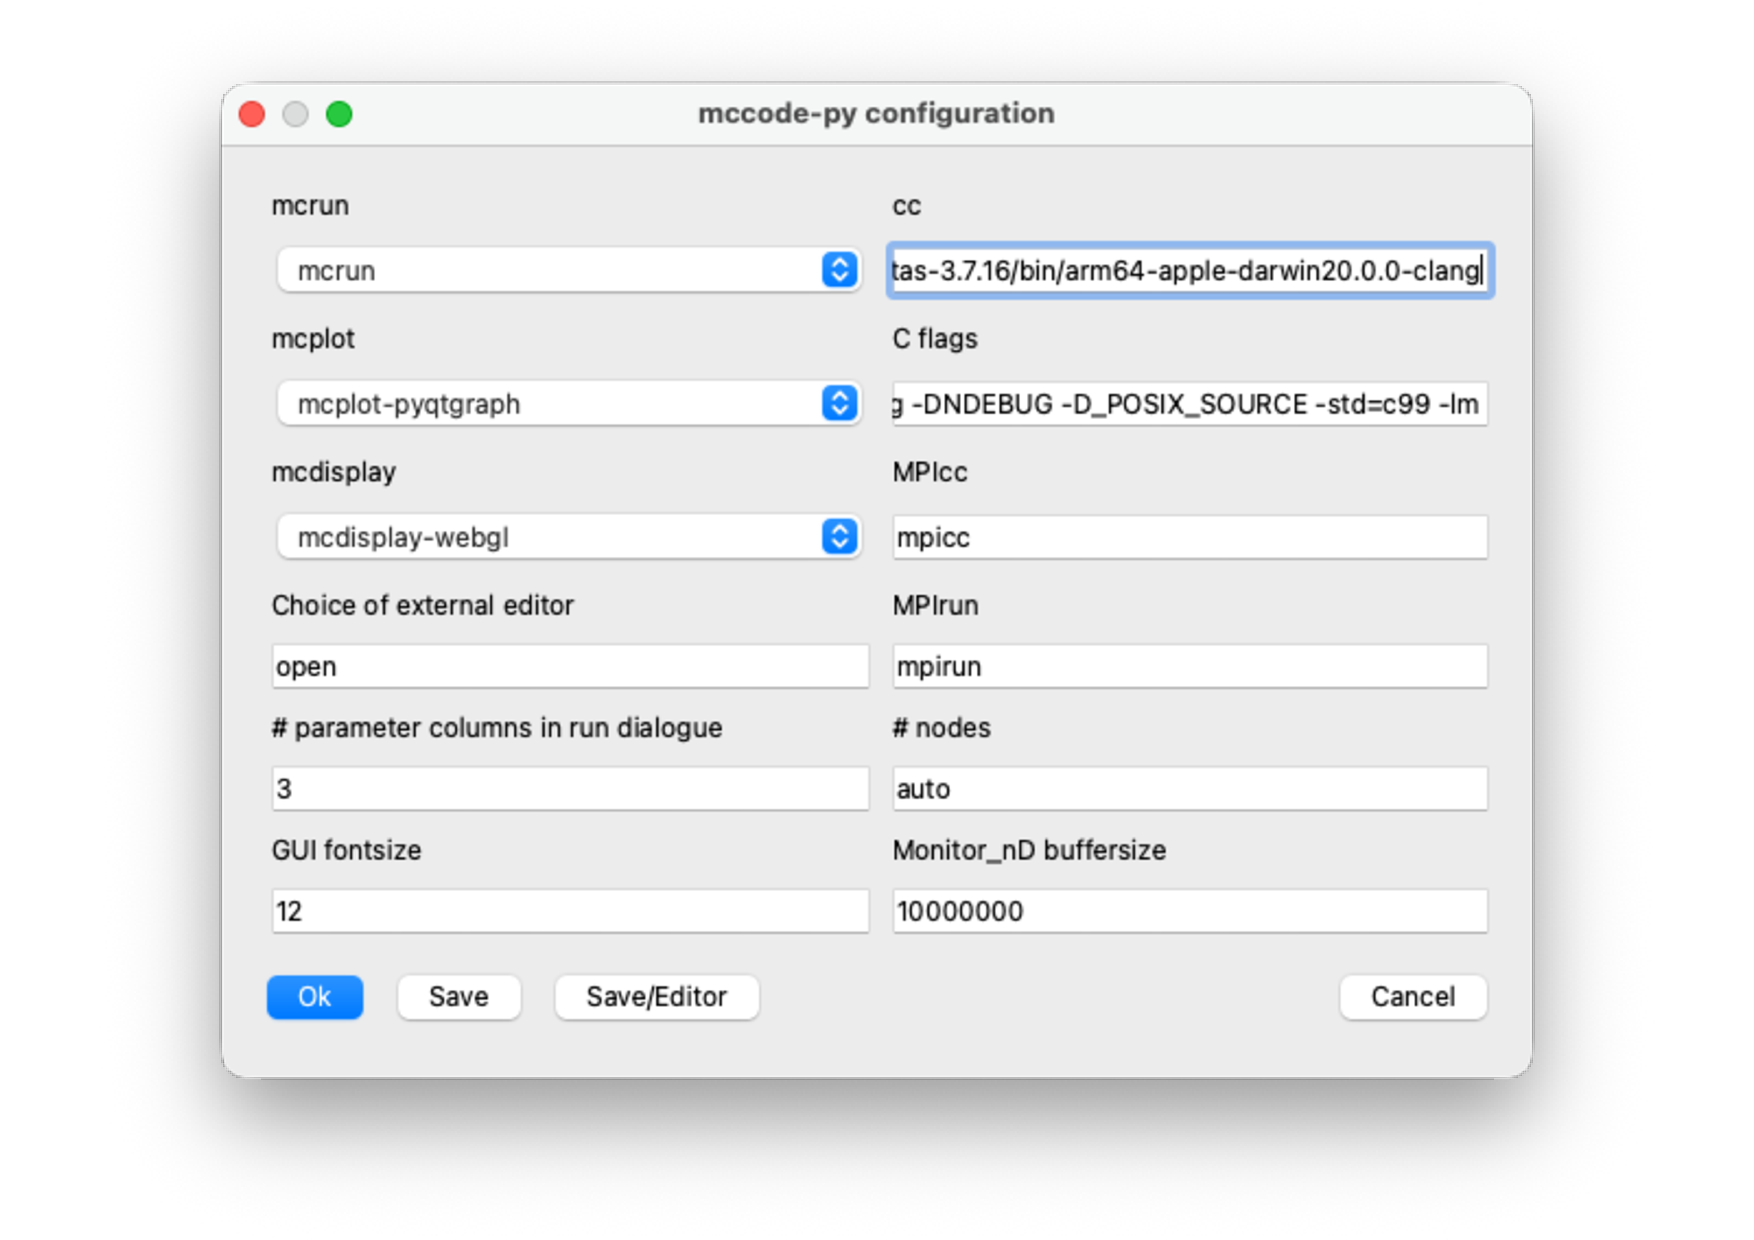
\includegraphics[width=0.75\textwidth]{figures/choose_backend}
  \end{center}
\caption{The ``configuration options'' dialog in \texttt{mcgui}.}
\label{fig:mcgui-choose}
\end{figure}


\noindent The \textbf{New from Template} menu (known as ``Neutron site'' in
older \MCS releases) contains a list of template and example
instruments as found in the \MCS library, sorted by category/facility (e.g.
\texttt{Templates}, \texttt{ILL}, \texttt{ISIS}, \texttt{ESS},
\texttt{Union\_demos}, \ldots -- see chapter~\ref{s:instrument} for a
curated tour). When
selecting one of these, a local copy of the instrument description is
transferred to the active directory (so that users have modification rights) and
loaded. One may then view its source (Edit) and use it directly for
simulations/trace (3D View).
\\\ \\

\noindent The \textbf{Tools} menu gathers minor tools.
\begin{description}
\item[Tools/Plot current/other results] Plot current simulation results and
  other results.
\item[Tools/Dataset convert/merge] Opens a GUI to merge scattered data sets
  (e.g. from successive runs or an MPI job) or assemble scan sets.
\item[Tools/Shortcut keys] displays the shortcut keys used for running and
  editing instruments.
\end{description}


\noindent The \textbf{Help} menu has the following features, through use of
\verb+mcdoc+ and a web browser. To customize the used web browser, set
the \verb+BROWSER+ environment variable. If \verb+BROWSER+ is not set,
\verb+mcgui+ uses \verb+netscape/mozilla/firefox+ on Unix/Linux and the default browser on
Windows.
\begin{description}
\item[Help/\MCS User manual] calls \verb+mcdoc --manual+, brings up the local
  pdf version of this manual, using a web browser.
\item[Help/\MCS Component manual] calls \verb+mcdoc --comps+, brings up the local
  pdf version of the component manual, using a web browser.
\item[Help/Component library index] displays the component documentation using
  the component \verb+index.html+ index file.
\item[Help/\MCS web page] calls \verb+mcdoc --web+, brings up the \MCS
  website in a web browser.
\item[Help/Tutorial] opens the \MCS tutorial for a quick start.
\item[Help/Current instrument info] generates a description web-page of the
  current edited instrument.
\item[Help/Test \MCS installation] launches \texttt{mctest} to check that
  the \MCS package is installed properly and generates accurate results
  (see section~\ref{s:frontends}).
\item[Help/Generate component index] (re-)generates locally the component
  \verb+index.html+.
\end{description}


\subsubsection{The run dialog}

\begin{figure}[htb!]
  \begin{center}
    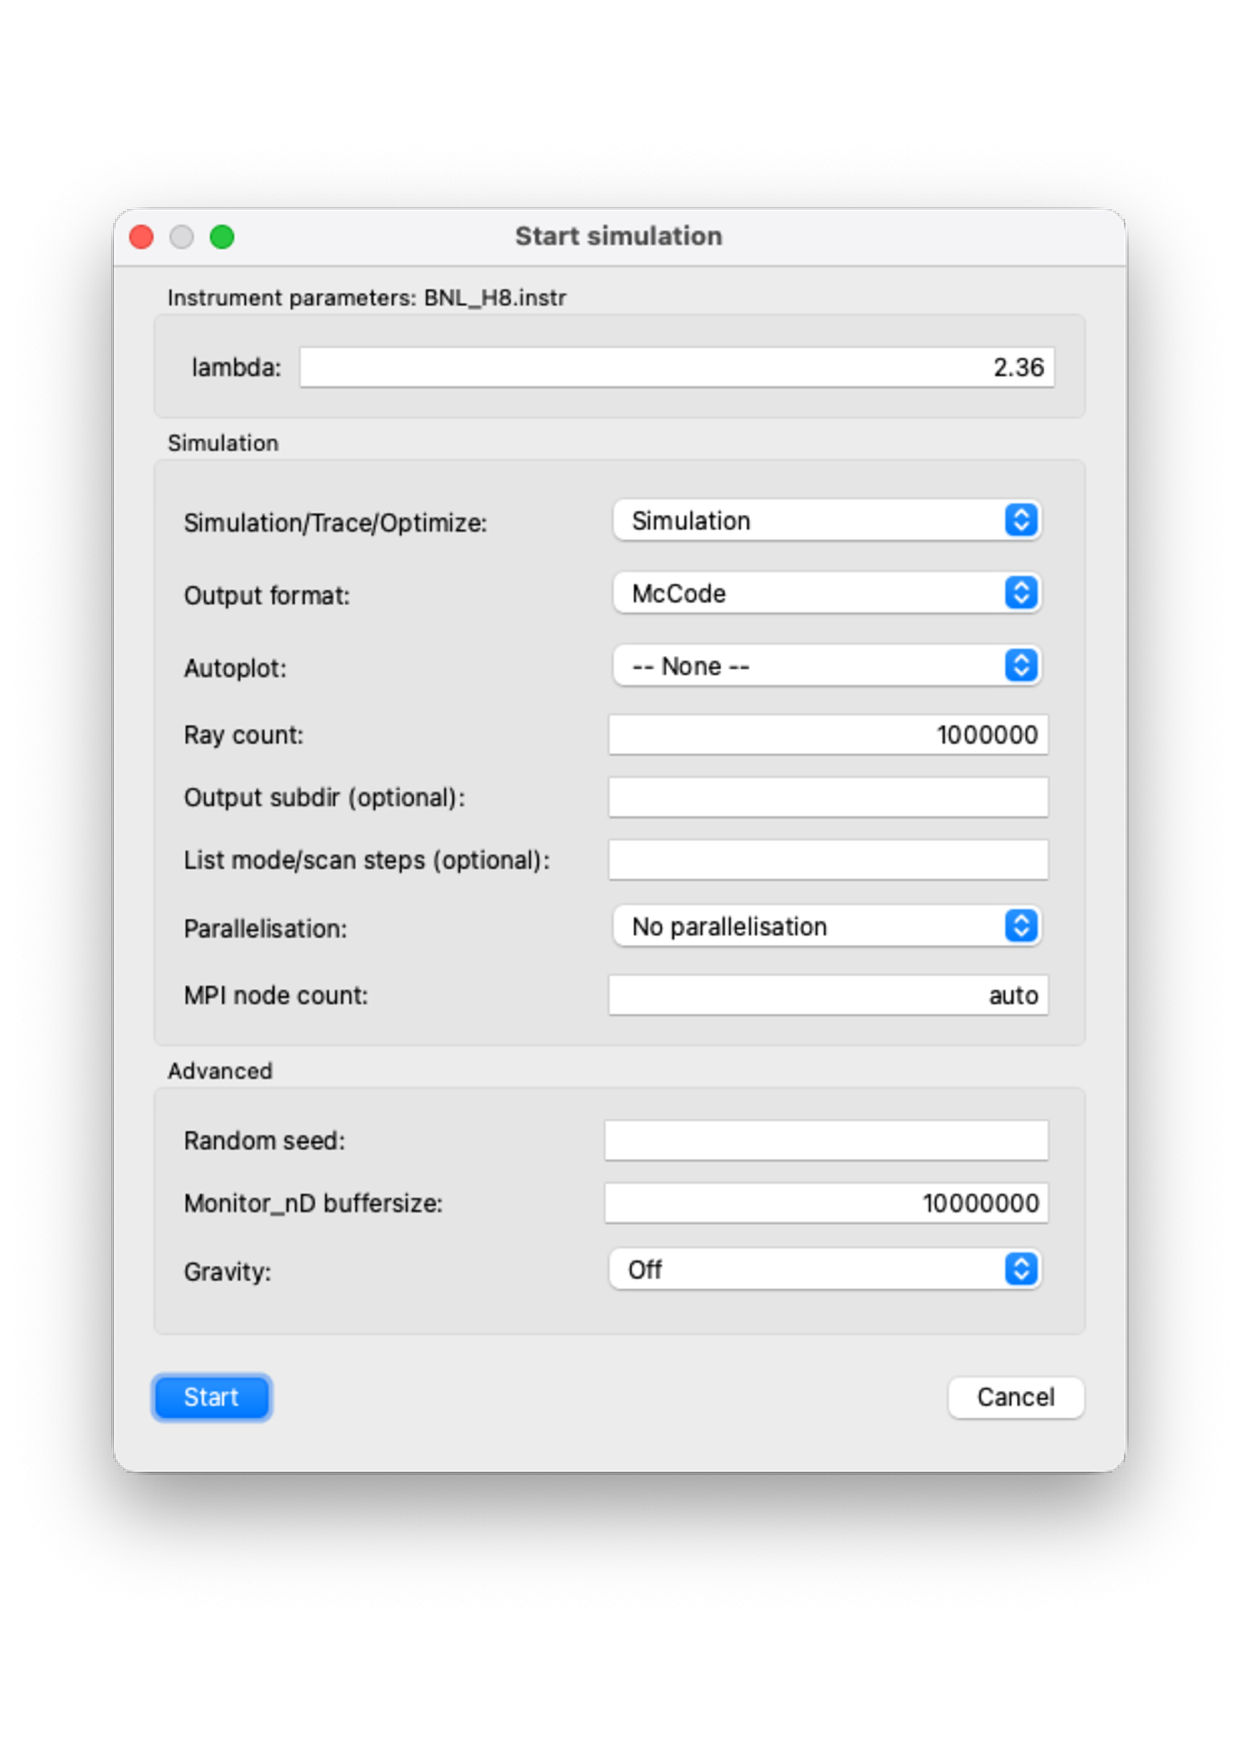
\includegraphics[width=0.75\textwidth]{figures/mcgui-run}
  \end{center}
\caption{The run dialog in \texttt{mcgui}.}
\label{fig:mcgui-run}
\end{figure}
%
The run dialog is used to run simulations. It allows the entry of instrument
parameters as well as the specifications of options for running the simulation
(see section~\ref{s:run-sim} for details). It also allows to run the
\verb+mcdisplay+ (section~\ref{s:mcdisplay}) and \verb+mcplot+
(section~\ref{s:mcplot}) front-ends together with the
simulation.\indexMCTOOL{mcplot}{}

The meaning of the different fields is as follows:
\begin{description}
\item[Run:Instrument parameters] allows the setting of the values for the input
  parameters of the instrument. The type of each instrument parameter is given
  in parenthesis after each name. Floating point numbers are denoted by (D) (for
  the C type ``\verb+double+''), (I) denotes integer parameters, and (S) denotes
  strings. For parameter scans and optimizations, enter the minimum and maximum
  values to scan/optimize, separated by a comma, e.g. \verb+1,10+ and do not
  forget to set the \textbf{\# Scanpoints} to more than 1.
\item[Run:Output to] allows the entry of a directory for storage of the
  resulting data files in (like the \verb+--dir+ option). If no name is given,
  the results are stored in the current directory, to be overwritten by the next
  simulation.
\item[Run:Force] Forces \MCS to overwrite existing data files
\item[Neutron count] sets the number of neutron rays to
  simulate (the \verb+--ncount+ option).
\item[Run:Gravity] Activates gravitation handling. Not all components full
  support the use of gravitation, but all transport in ``free space'' using the
  PROP\_DT, PROP\_Z0 etc. macros will include propagation with gravity. Only
  local, internal component propagation without the PROP routines will be
  gravity-less. As a conclusion it is considered safe and to high precision
  correct to apply the gravitation setting if one takes care to use the
  Guide\_gravity component and other gravity-supporting guide types in
  combination with non-gravity components that are ``small'' in size,
  i.e. samples, lenses, etc.
\item[Run:Random seed/Set seed to] selects between using a random seed (different
  in each simulation) for the random number generator, or using a fixed
  seed (to reproduce results for debugging).
\item[Run:Simulate/Trace (3D)/Optimize] selects between several modes of
  running the simulation:
  \begin{itemize}
  \item Simulate: perform a normal simulation or a scan when \#steps
    is set to non-zero value
  \item Trace (3D view): View the instrument in 3D tracing individual
    neutrons through the instrument
  \item Optimize: find the optimum value of the simulation parameters
    in the given ranges (see section \ref{s:optimize}).
  \item Backgrounding (bg): Simulate or Optimize in the background.
\end{itemize}
\item[Run:\# steps / \# optim] sets the number of simulation to run when
  performing a parameter scan or the number of iterations to
  perform in optimization mode.
\item[Run:Plot results] -- if checked, the \verb+mcplot+ front-end will be run
  after the simulation has finished, and the plot dialog will appear
  (see below).
\item[Run:Format] quick selection of output format (\texttt{McCode} or
  \texttt{NeXus}).
\item[Run:Clustering method] selects between running locally or via MPI.
  See section~\ref{s:run-mpi} on parallel computing for
  more informations.
\item[Run:Number of nodes] sets the number of MPI nodes to use.
\item[Run:Inspect component] (Trace mode) will trace only neutron trajectories
  that reach a given component (e.g. sample or detector).
\item[Run:First component] (Trace mode) seletcs the first component to plot
  (default is first) in order to define a region of interest.
\item[Run:Last component] (Trace mode) seletcs the last component to plot
  (default is first) in order to define a region of interest.
\item[Run:Maximize monitor] (Optimization mode) seletcs up to three monitors
  which integral value should be maximized, varying instrument parameters. If no
  monitor is selected, the sum of all monitors is optimized.
\item[Run:Start] runs the simulation.
\item[Run:Cancel] aborts the dialog.
\end{description}
Most of the settings on the run dialog can be saved for your next
\MCS run using 'Save configuration' in the File menu.

Before running the simulation, the instrument definition is automatically
compiled if it is newer than the generated C file (or if the C file is newer
than the executable). The executable is assumed to have a \verb+.out+ suffix in
the filename. NB: If components are changed, automatic compilation is \emph{not}
performed. Instead, use the File/Compile menu item in mcgui.



\subsubsection{The editor window}

The editor window provides a simple editor for creating and modifying instrument
definitions. Apart from the usual editor functions, the ``Insert'' menu provides
some functions that aid in the construction of the instrument definitions:
\begin{description}
\item[Editor Insert/Instrument template] inserts the text for a simple instrument
  skeleton in the editor window.
\item[Editor Insert/Component\ldots] opens up a dialog window with a list of all
  the components available for use in \MCS. Selecting a component will
  display a description. Double-clicking will open up a dialog window
  allowing the entry of the values of all the parameters for the
  component (figure~\ref{f:comp_dialog}). See section~\ref{s:instrdefs}
  for details of the meaning of the different fields.

  The dialog will also pick up those of the users own components that are
  present in the current directory when \verb+mcgui+ is started. See
  section~\ref{s:mcdoc} for how to write components to integrate well with this
  facility.
\item[Editor Insert/\textit{Type}] These menu entries give quick access to the
  entry dialog for the various component types available, i.e. Sources, Optics,
  Samples, Monitors, Misc, Contrib and Obsolete.
\end{description}
\begin{figure}[tbp]
  \begin{center}
    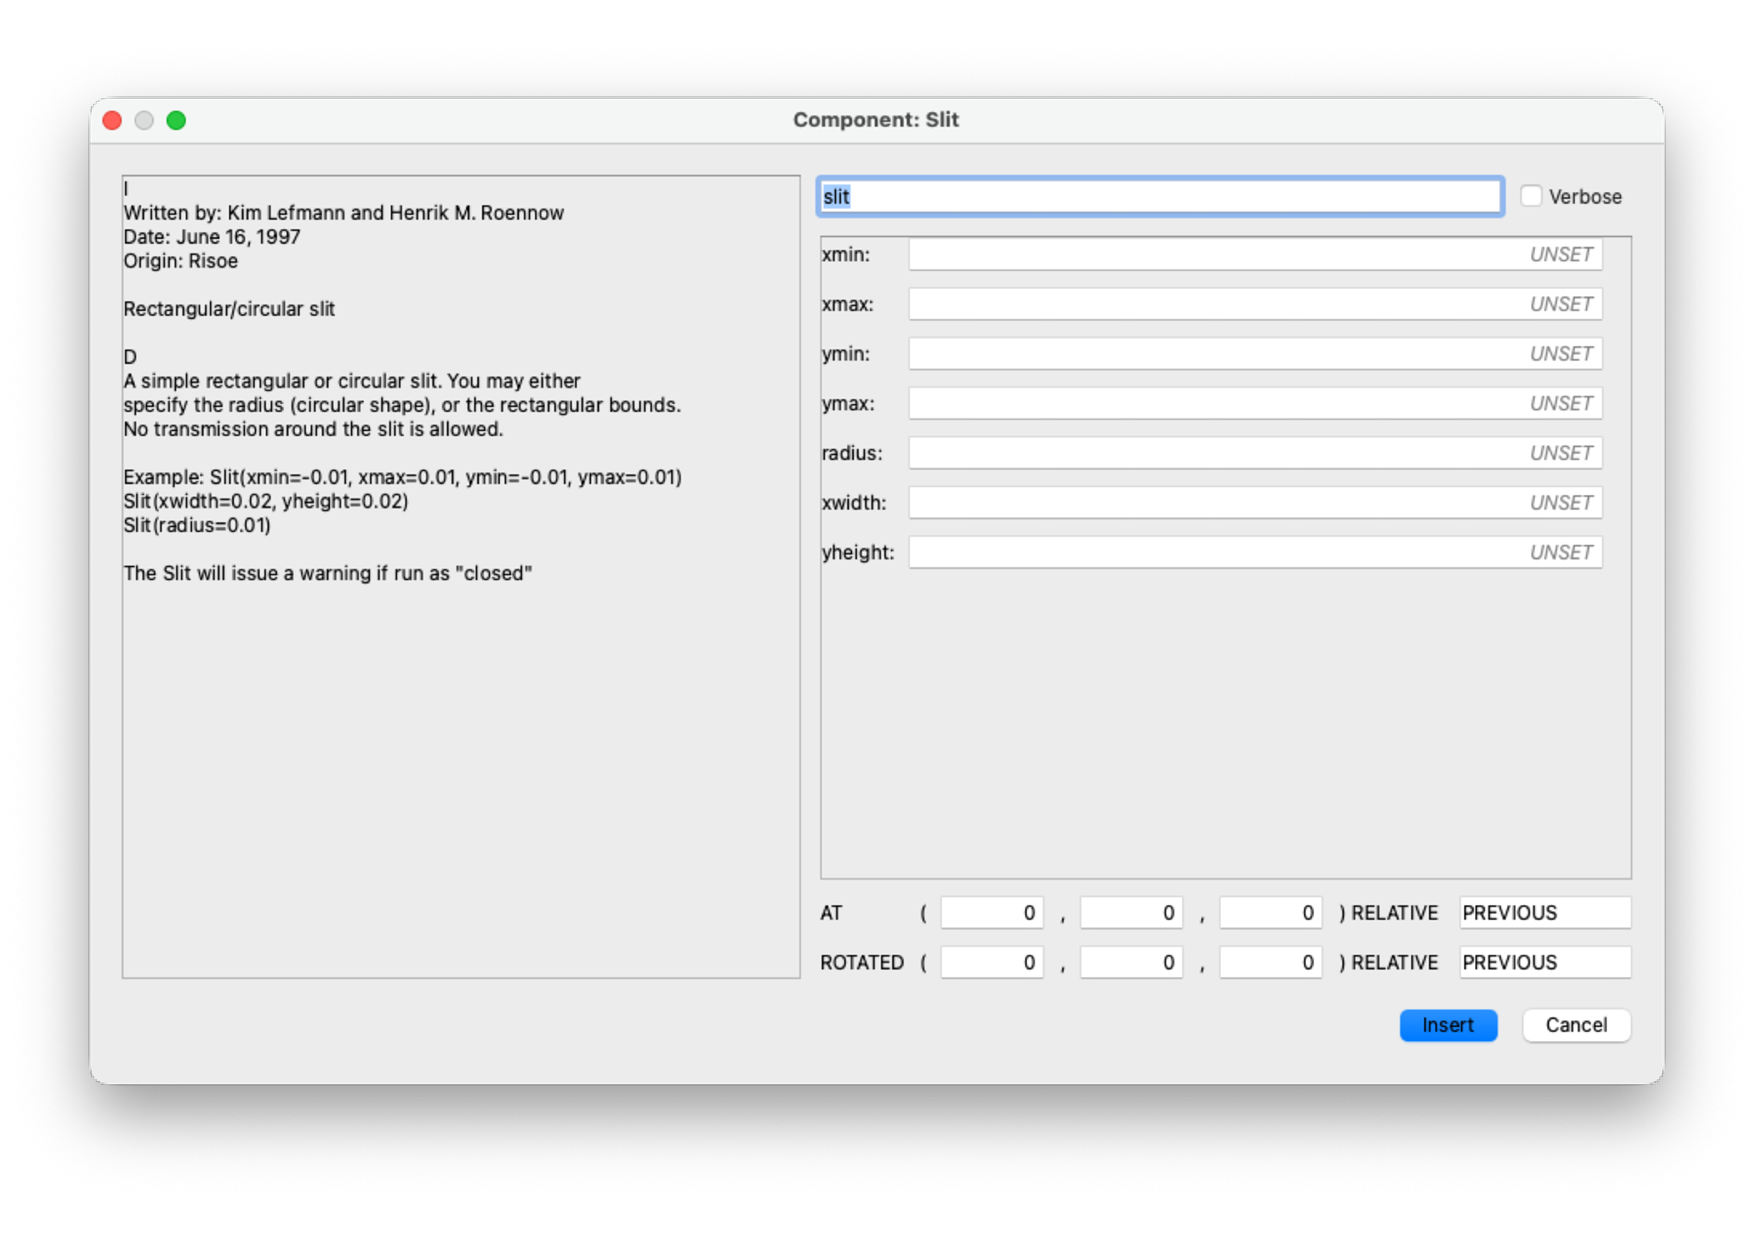
\includegraphics[width=0.75\textwidth]{figures/comp_dialog}
    \caption{Component parameter entry dialog.}
    \label{f:comp_dialog}
  \end{center}
\end{figure}


%-------------------------------------------------------------------------------
\subsection{Running simulations on the commandline (mcrun)}
\label{s:mcrun}
\indexMCTOOL{mcrun}{textbf}
\index{Parameters!instruments}
\index{Parameters!scans}
\index{Parameters!optimization}

The \verb+mcrun+ front-end provides a convenient
command-line interface for running simulations with the same automatic
compilation features available in the \verb+mcgui+ front-end. It also provides a
facility for running a series of simulations while varying an input parameter.

The command

\begin{bash}
mcrun sim args ...
\end{bash}

will compile the instrument definition \texttt{\textit{sim}.instr} (if
necessary) into an executable simulation \texttt{\textit{sim}.out}. It
will then run \texttt{\textit{sim}.out}, passing the argument list \textit{
  args}

The possible arguments are the same as those accepted by the simulations
themselves as described in section~\ref{s:run-sim}, with the following
extensions:
\begin{itemize}
\item The \verb+-c+ or \verb+--force-compile+ option may be used to force the
  recompilation of the instrument definition, regardless of file dates. This may
  be needed in case any component definitions are changed (in which case
  \verb+mcrun+ does not automatically recompile), or if a new version of \MCS
  has been installed.
\item The \texttt{-p \textit{file}} or \texttt{--param=\textit{file}} option may be
  used to specify a file containing assignment of values to the input parameters
  of the instrument definition. The file should consist of specifications of the
  form \texttt{\textit{name\/}=\textit{value\/}} separated by spaces or line
  breaks. Multiple \verb+-p+ options may be given together with direct parameter
  specifications on the command line. If a parameter is assigned multiple times,
  later assignments override previous ones.
\item The \texttt{-N \textit{count}} or \texttt{--numpoints=\textit{count}} option
  may be used to perform a series of \textit{count\/} simulations while
  varying one or more parameters within specified intervals. Such a
  series of simulations is called a \emph{scan}. To specify
  an interval for a parameter \textit{X}, it should be assigned two
  values separated by a comma. For example, the command
\begin{bash}
mcrun sim.instr -N4 X=2,8 Y=1
\end{bash}
would run the simulation defined in \verb+sim.instr+ four times, with
\textit{X} having the values 2, 4, 6, and 8, respectively.

After running the simulation, the results will be written to the file
\verb+mccode.dat+ by default (see the \verb+--optimise-file+ option). This
file contains one line for each simulation
run giving the values of the scanned input variables along with the integrated
intensity and estimated error in all monitors. This file can be plotted with
any of the \verb+mcplot+ backends, see section~\ref{s:mcplot}.
\indexMCTOOL{mcplot}{}
\item When performing a scan, the \texttt{-f \textit{file}} and
  \texttt{--file=\textit{file}} options make \verb+mcrun+ write the output
  to the files \texttt{\textit{file\/}.dat} and \texttt{\textit{file\/}.sim}
  instead of the default names.
\item When performing a scan, the \texttt{-d \textit{dir}} and
  \texttt{--dir=\textit{dir}} options make \verb+mcrun+ put all output in a
  newly created directory \textit{dir}. Additionally, the directory will
  have subdirectories \verb+1+, \verb+2+, \verb+3+,\ldots containing all
  data files output from the different simulations. When the \verb+-d+
  option is not used, no data files are written from the individual
  simulations (in order to save disk space).
\end{itemize}

The \verb+-h+ option will list valid options; see also Table~\ref{f:mcrunoptions}
for the complete, current option list.

\subsection{GPU acceleration via OpenACC}
\label{s:gpu}

\MCS~3.x supports GPU-accelerated simulations through the OpenACC
framework, enabling substantial speed-ups over CPU-only execution on
compatible NVIDIA hardware.

\subsubsection{Requirements}

\begin{itemize}
  \item \textbf{Compiler:} NVIDIA HPC SDK version~20.x or newer.  The
        free Community Edition is sufficient.
  \item \textbf{Hardware:} A CUDA-capable NVIDIA GPU with an up-to-date
        driver.
  \item \textbf{Platform:} GPU support is currently available on Linux
        only.  Windows is not yet supported for OpenACC by NVIDIA; Windows
        users wishing to use GPU acceleration should do so via
        WSL~2 running a Linux distribution.
\end{itemize}

\subsubsection{Running a GPU-accelerated simulation}

Pass the \verb+--openacc+ flag to \texttt{mcrun}:
\begin{verbatim}
  mcrun --openacc MyInstrument.instr -n 1e9
\end{verbatim}

\paragraph{Combined multi-core + GPU execution.}
It is also possible to use both CPU cores and the GPU simultaneously.
Enable this by adding the following to the \texttt{OACCFLAGS} field of
your \texttt{mccode\_config.json}:
\begin{verbatim}
  "OACCFLAGS": "-fast -Minfo=accel -acc=gpu,multicore
                -gpu=managed -DOPENACC -DMULTICORE"
\end{verbatim}

\subsubsection{Further information}

GPU terminology specific to \MCS/McXtrace~3 and detailed debugging
tips are documented on the McCode wiki:
\begin{itemize}
  \item GPU terminology table:\\
    \url{https://github.com/mccode-dev/McCode/wiki/McStas-McXtrace-3-and-GPU-terminology-(table)}
  \item GPU debugging tips:\\
    \url{https://github.com/mccode-dev/McCode/wiki/GPU-Debugging-tips}
\end{itemize}



%-------------------------------------------------------------------------------
\subsection{Graphical display of simulations (mcdisplay)}
\label{s:mcdisplay}
\indexMCTOOL{mcdisplay}{textbf}

The front-end \verb+mcdisplay+ is a graphical
visualization tool, very useful for debugging.  It presents a schematic drawing
of the instrument definition, showing the position of the components and the
paths of the simulated neutrons through the instrument. It is thus very useful
for debugging a simulation, for example to spot components in the wrong position
or to find out where neutrons are getting lost.

To use the \verb+mcdisplay+ front-end with a simulation, run it as
follows:
\begin{bash}
mcdisplay sim args ...
\end{bash}

where \verb+sim+ is the name of either the instrument source
\texttt{\textit{sim}.instr} or the simulation program \texttt{\textit{sim}.out} generated by \mcs,
and \textit{args \ldots} are the normal command line arguments for the
simulation, as explained above. The \verb+-h+ option will list valid options.

The drawing back-end may be selected by invoking one of the dedicated
front-ends directly:
\begin{itemize}
\item \verb+mcdisplay-pyqtgraph+ (the default when running plain
  \verb+mcdisplay+): interactive PyQtGraph 3D view.
\item \verb+mcdisplay-matplotlib+: static/interactive matplotlib 3D view.
\item \verb+mcdisplay-webgl+ and \verb+mcdisplay-webgl-classic+: browser-based
  WebGL views (the former uses a small NodeJS-backed server for larger
  instruments/particle counts).
\item \verb+mcdisplay-cad+: exports the instrument geometry to a CAD-compatible
  format.
\item \verb+mcdisplay-mantid_xml+: exports an approximate Mantid Instrument
  Definition File (IDF) describing the detector geometry.
\end{itemize}
For instance, calling
\begin{bash}
mcdisplay-webgl BNL_H8.instr lambda=2.36
\end{bash}
will open a WebGL view of the instrument in a browser tab.
The \verb+mcdisplay+ front-end can also be run from the \verb+mcgui+ front-end.
\indexMCTOOL{mcgui}{}

The (default, PyQtGraph) front-end accepts the following options, amongst
others -- run \verb+mcdisplay --help+ for the complete, current list:
\begin{itemize}
\item \verb+--default+: automatically use the instrument's default parameter
  values, without prompting.
\item \verb+--dirname=DIR+: override the output directory name used while
  tracing.
\item \verb+--inspect=+\textit{comp}: only display neutron trajectories that
  reach the component named \textit{comp}. This is useful when debugging, e.g.
  to hide neutrons absorbed upstream of the component of interest.
\item \verb+--invcanvas+: invert the canvas background from black to white
  (useful for printing or screenshots).
\item \verb+-n+/\verb+--ncount=N+: number of neutron rays to trace.
\end{itemize}

When debugging trajectories through a long or complex instrument, combining
\verb+--inspect+ with a modest \verb+--ncount+ typically gives the clearest,
fastest picture of what is happening around a particular component.

%-------------------------------------------------------------------------------
\subsection{Plotting the results of a simulation (mcplot)}
\label{s:mcplot}
\indexMCTOOL{mcplot}{textbf}

The front-end \verb+mcplot+ is a program that produces
plots of all the monitors in a simulation, and it is thus useful to get
a quick overview of the simulation results.

In the simplest case, the front-end is run simply by typing
\begin{bash}
    mcplot
\end{bash}
This will plot any simulation data stored in the current directory, which is
where simulations store their results by default. If the \verb+--dir+ or
\verb+--file+ options have been used (see section~\ref{s:run-sim}), the name of
the file or directory should be passed to mcplot, {\em e.g.} ``\texttt{mcplot
  \textit{dir}}'' or ``\texttt{mcplot \textit{file}}''.  It is also possible to plot
one single text (not binary) data file from a given monitor, passing its name to
mcplot.

As with \texttt{mcdisplay} (section~\ref{s:mcdisplay}), the drawing back-end
may be selected by invoking the dedicated front-end directly:
\verb+mcplot-pyqtgraph+ (the default), \verb+mcplot-matplotlib+, or
\verb+mcplot-html+ (renders an interactive, self-contained web page using
D3.js, see section~\ref{s:run-format}), or by setting the
\verb+MCSTAS_FORMAT+ environment variable.
\indexEV{MCSTAS\_FORMAT}

All plotters read the plain-text \MCS/McCode data format (section~\ref{s:analyze});
NeXus files are not currently read back by the plotters.

The \verb+mcplot+ front-end can also be run from the \verb+mcgui+ front-end.
\indexMCTOOL{mcgui}{}

The initial display shows plots for each detector in the simulation.

\paragraph{Comparing two simulation results: mcplotdiff-html and mccoplot-html.}
\indexMCTOOL{mcplotdiff}{textbf}
\indexMCTOOL{mccoplot}{textbf}
Two companion browser-based tools reuse \texttt{mcplot-html}'s plotting code to
compare a pair of simulation results (two output directories, or two single
monitor files), matching monitors by output filename:
\begin{itemize}
\item \verb+mcplotdiff-html a b+ plots, for every monitor present with
  matching binning in both \texttt{a} and \texttt{b}, the difference
  \texttt{a - b} (with error-propagated error bars for 1D monitors, and a
  diverging blue/white/red colour scale for 2D monitors). This is useful to
  quickly spot the effect of a component or parameter change, an \MCS version
  upgrade, or MPI vs.\ non-MPI results. By default, each difference is also
  written back out as a normal \MCS/McCode-format data set (with an
  \texttt{mccode.sim} index), so the result directory can be reopened by any
  other McCode-format-aware plotter; pass \verb+--no-dat+ to skip this.
\item \verb+mccoplot-html a b+ instead overlays the two datasets' 1D monitors
  on the same axes (only 1D monitors are supported), for a direct visual
  comparison of curve shape and position.
\end{itemize}
Both accept \verb+-A LABEL_A+/\verb+-B LABEL_B+ to control the labels used for
each input, and \verb+-o OUTPUT+ to control the output directory name; run
either with \verb+--help+ for the complete option list. \texttt{mcplotdiff-html}
is also used internally by \texttt{mcviewtest} (section~\ref{s:frontends}) to
compare test runs against a reference.


%-------------------------------------------------------------------------------
\subsection{Plotting resolution functions (mcresplot)}
\label{s:mcresplot}
\indexMCTOOL{mcresplot}{textbf}

The \verb+mcresplot+ front-end is used to plot the resolution function,
particularly for triple-axis
spectrometers, as calculated by the Res\_sample component or TOF\_Res\_sample
for time-of-flight instruments. It requires to have a Res\_monitor (or
TOF\_Res\_monitor) component further in the instrument description (at the
detector position).

As of \MCS 3.x, \verb+mcresplot+ is a pure Python tool built around a
covariance-matrix method (rather than reading a resolution ellipsoid
directly out of the simulation), following the approach implemented in the
Takin2 package~\cite{takin2}. Neutron events collected by the Res\_monitor
are loaded with NumPy, the weighted covariance matrix of the
$(\boldsymbol{Q},\omega)$ four-vectors is computed and inverted to obtain
the resolution matrix, and the resulting ellipsoids are drawn with
\texttt{matplotlib} (2D projections and slices, plus a 3D view).

The \verb+mcresplot+ front-end is launched with the command
\begin{lstlisting}
mcresplot outfile
\end{lstlisting}
Here, \textit{outfile\/} is the name of a file output from a simulation using
the Res\_monitor component. Useful options include \verb+--QEfile+ (if the
event file is in the $h\,k\,l\,E\,w$ format rather than the default
$\mathbf{k}_i\,\mathbf{k}_f\,w_i\,w_f$ format), \verb+--centreonQ+ (center
plots on the mean $\boldsymbol{Q}$ rather than the origin), \verb+--save=file+
(save the plots to a file instead of, or in addition to, showing them
interactively), \verb+--noplot+ (compute and print the resolution matrices
only, without opening a plot window) and \verb+--tex+ (use \LaTeX{} for axis
labels). Run \verb+mcresplot --help+ for the full, current option list.

The front-end will open a window displaying projections of the 4-dimensional
resolution function $R(\boldsymbol{Q}, \omega)$, measured at a
particular choice of $\boldsymbol{Q}$ and $\omega$, see the component
manual. The covariance matrix of the
resolution function, the resolution along each projection axis and the resulting
resolution matrix are also shown, as well as the instrument name and parameters
used for the simulation.

To use the \verb+mcresplot+ front-end, a Python installation with NumPy and
matplotlib is required (both are part of the standard \MCS conda-forge
environment).

%-------------------------------------------------------------------------------
\subsection{Creating and viewing the library, component/instrument help and
  Manuals (mcdoc)}
\label{s:mcdoc-run}
\indexMCTOOL{mcdoc}{textbf}

\MCS provides an easy way to generate automatically an HTML help page about a
given component or instrument, or the whole \MCS
library. \index{Library!components}
\begin{lstlisting}
mcdoc
mcdoc searchterm
mcdoc file.comp
\end{lstlisting}
The first example generates an \textit{index.html} catalog file using the available
components and instruments (both locally, and in the \MCS library), and browses
it using the \verb+BROWSER+ environment variable
\indexEV{BROWSER}
(e.g. firefox, chromium, \ldots). Alternatively, if a search term or a
\textit{file.comp}/\textit{file.instr} path is given, \verb+mcdoc+ will
search within the library and open documentation for all matching entries.

Additional options include \verb+--install+/\verb+-i+ (regenerate the local
installation-wide index), \verb+--dir=DIR+/\verb+-d+ (add search results from
a given directory), and \verb+--verbose+/\verb+-v+ (print a parsing log).
The options \verb+--manual+/\verb+-m+, \verb+--comps+/\verb+-c+ and
\verb+--web+/\verb+-w+ will open the User Manual (this document), the
Component Manual, and the \MCS web site, respectively, all requiring
\verb+BROWSER+ to be defined. Finally, the \verb+--help+
option will display the command help, as usual.

See section~\ref{s:mcdoc} for more details about the McDoc usage and header
format.  \verb+mcdoc+ is a pure Python tool, part of the standard \MCS
conda-forge package.

\paragraph{Online wiki.}
In addition to this manual, extensive and frequently updated documentation
is maintained on the McCode GitHub wiki~\cite{Wiki}:
\begin{center}
  \url{https://github.com/mccode-dev/McCode/wiki}
\end{center}
The wiki includes end-user guides, component development howtos, GPU
acceleration information, and migration guides from \MCS~2.x to 3.x.


%-------------------------------------------------------------------------------
\subsection{Self-testing the installation (mctest, mcviewtest)}
\label{s:mctest}
\indexMCTOOL{mctest}{textbf}
\indexMCTOOL{mcviewtest}{textbf}

\MCS ships with a Python self-test/benchmark harness, replacing the earlier
\verb+mcrun --test+ command. \verb+mctest+ compiles and runs a selection (or
all) of the example instruments found under the current installation(s), and
stores each run's results (including any test-defined \texttt{\%Example}
reference values) in a timestamped output folder. Useful options include
\verb+--ncount+, \verb+--mpi+ and \verb+--openacc+ (forwarded to \verb+mcrun+
for every tested instrument), \verb+--config=LABEL+ (test only a specific
McCode installation/config), \verb+--instr=REGEX+ (test only matching
instrument names), and \verb+--limit=N+ (test only the first N instruments
per version); run \verb+mctest --help+ for the full list.

\verb+mcviewtest+ then generates an HTML report of one or more \verb+mctest+
runs found in a given folder (the current directory by default). When more
than one run is present (e.g. a reference run and a run on a different
platform, GPU vs.\ CPU, or a different \MCS branch), it takes the oldest
subfolder as the reference column, and additionally runs
\texttt{mcplotdiff-html} (section~\ref{s:mcplot}) between each other column's
monitor output and the reference's, adding a \texttt{DIFF~[vs~ref]} link next
to each such row in the report. These comparisons are cached on disk and
generated in parallel (\verb+--diffworkers+), so re-running \verb+mcviewtest+
is fast; use \verb+--nodiff+ to skip generating them entirely, or
\verb+--diff-errors-only+ to only diff rows that already show a discrepancy.

%%%%%%%%%%%%%%%%%%%%%%%%%%%%%%%%%%%%%%%%%%%%%%%%%%%%%%%%%%%%%%%%%%%%%%%%%%%%%%%%
\section{Data formats - Analyzing and visualizing the simulation results}
\label{s:analyze}
\index{Data formats}

To analyze simulation results, one uses the same tools as for analyzing
experimental data, \textit{i.e}. programs such as Python/NumPy, Matlab, IDL.  The
output files from simulations are usually simple text files containing headers
and data blocks. If data blocks are empty they may be accessed referring to an
external file indicated in the header.

Each data file contains information about the simulation, the instrument, the
parameters used, and of course the signal, the estimated error on the signal,
and the number of events used in each bin. Additionally, all data files indicate
their first moment (mean value) and second moment (half width) in the
'statistics' field.

The available data formats are the legacy \MCS (McCode) format, and the HDF/NeXus binary when the needed libraries are installed.
\indexEV{MCSTAS\_FORMAT}

In order for the user to choose the data format, we recommend to set it using
the \verb+--format=FORMAT+ or alternatively \textit{via} the MCSTAS\_FORMAT
environment variable, which will also make the front-end programs able to import
and plot data and instrument consistently (see Section \ref{s:run-sim}). 

Note that the neutron event counts in detectors are typically not very
meaningful except as a way to measure the performance of the
simulation. Use the simulated intensity instead whenever analyzing
simulation data.

%-------------------------------------------------------------------------------
\subsection{The \MCS/McCode text format}
\index{Data formats}
The \MCS original format, sometimes still referred to by its historical name
``PGPLOT format'' (the plotting package used in \MCS~1.x/2.x), is simply
columns of ASCII text that most
programs should be able to read.

One-dimensional histogram monitors (time-of-flight, energy)
write one line for each histogram bin. Each line contains a number
identifying the bin (\textit{i.e}.\ the time-of-flight) followed by
three numbers: the simulated intensity, an estimate of the statistical
error as explained in section~\ref{s:staterror}, and the number of
neutron events for this bin.

Two-dimensional histogram monitors (position sensitive detectors) output $M$
lines of $N$ numbers representing neutron intensities, where $M$ and $N$ are the
number of bins in the two dimensions. The two-dimensional monitors also store
the error estimates and event counts as additional matrices.

Single-point monitors output the neutron intensity, the estimated
error, and the neutron event count as numbers on the
terminal. (The results from a series of simulations may be combined in a
data file using the \verb+mcrun+ front-end as explained in
section~\ref{s:mcrun}).

When using one- and two-dimensional monitors, the integrated intensities are
written to terminal as for the single-point monitor type, supplementing file
output of the full one- or two-dimensional intensity distribution. Both one- and
two-dimensional monitor output by default start with a header of comment lines,
all beginning with the `\verb+#+' character.  This header gives such information
as the name of the instrument used in the simulation, the values of any
instrument parameters, the name of the monitor component for this data file,
\textit{etc}. The headers may be disabled using the \verb+--data-only+ option in
case the file must be read by a program that cannot handle the headers.

In addition to the files written for each one- and two-dimensional monitor
component, another file (by default named \verb+mccode.sim+) is also
created. This file is in a special \MCS ASCII format. It contains all available
information about the instrument definition used for the simulation, the
parameters and options used to run the simulation, and the monitor components
present in the instrument. It is read by the \verb+mcplot+ front-end (see
section~\ref{s:mcplot}). This file stores the results from single monitors, but
by default contains only pointers (in the form of file names) to data for one-
and two-dimensional monitors. By storing data in separate files, reading the
data with programs that do not know the special \MCS file format is
simplified. The \verb+--file+ option may be used to store all data inside the
\verb+mccode.sim+ file instead of in separate files.

%-------------------------------------------------------------------------------
\subsection{NeXus format}
\indexTOOL{NeXus}
\index{Data formats}
\label{r:nexus}

The NeXus format~\cite{nexus_webpage} is a platform independent HDF binary data
file. To have \MCS use it
\begin{enumerate}
\item the HDF and NeXus libraries must have been installed (libNeXus and headers)
\item the compilation of instruments must be done with the
  \verb+-DUSE_NEXUS -lNeXus+ flag (see Section \ref{s:nexus}). This is
  automated with the \verb+mcrun+ tool (Section \ref{s:mcrun}).
\end{enumerate}
All results are saved in a single file, containing 'groups' of data. To view
such files, install and use HDFView (or alternatively HDFExplorer). This Java
viewer can show content of all detectors, including metadata (attributes). Basic
detector images may also be generated.

%%%%%%%%%%%%%%%%%%%%%%%%%%%%%%%%%%%%%%%%%%%%%%%%%%%%%%%%%%%%%%%%%%%%%%%%%%%%%%%%
\section{Using MPI for parallel computing}
\label{s:run-mpi}
\index{Parallel computing|textbf}
\index{MPI|textbf}

Parallelizing a computation is in general possible when dependencies between
  each computation are not too strong. The situation of \MCS is
  ideal since each neutron ray can be simulated without interfering with
  other simulated neutron rays. Therefore each neutron ray can be simulated
  independently on a set of computers.

  When computing $N$ neutron rays with $p$ computers, each computer will
  simulate $\frac{N}{p}$ neutrons. As a result there will be $p \cdot
  \frac{N}{p} = N$ neutrons simulated. As a result, \MCS generates two kinds of
  data sets:
\begin{itemize}
\item intensity measurements, internally represented by three
  values $(p_0, p_1, p_2)$ where $p_0$, $p_1$, $p_2$ are
  additive. Therefore the final value of $p_0$ is the sum of all
  local value of  $p_0$ computed on each node. The same rule applies
  for $p_1$ and $p_2$. The evaluation of the intensity errors $\sigma$
  is performed using the final $p_0$, $p_1$, and $p_2$ arrays (see Section \ref{s:staterror}).
\item event lists: the merge of events is done by concatenation
\end{itemize}

\MCS provides two methods in order to distribute computations on many
computers.
\begin{itemize}
\item when using an homogeneous computer cluster, each simulation (including
  scan steps) may be computed in parallel using MPI. We recommend this method on
  clusters (see section \ref{s:mpi}).
\item \texttt{mcrun}'s built-in scan-splitting (\verb+--scan_split=N+, see
  Table~\ref{f:mcrunoptions}) distributes the individual steps of a parameter
  scan across \texttt{N} local CPU cores/threads, without requiring MPI. This
  is a lightweight alternative on a single multi-core machine.
\end{itemize}

All of these methods can be used, when available, from \texttt{mcgui}.

%-------------------------------------------------------------------------------
\subsection{Parallel computing (MPI)}
\index{MPI|textbf}

\label{s:mpi}
The MPI support requires that an MPI implementation (MPICH or OpenMPI are
both known to work) is installed on a set of nodes, together with a
properly configured passwordless \texttt{ssh} between nodes if running
across more than one machine.

There are 2 methods for using MPI
\begin{itemize}
\item Basic usage requires to compile and run the simulation by hand (mpicc, mpirun).
\item A much simpler way is to use \verb+mcrun -c --mpi=NB_CPU ...+ which will
  recompile and run with MPI support.
\item The McGUI interface also supports MPI from within the Run Dialog.
\end{itemize}

The MPI support is especially suited on clusters.

\subsubsection{Requirements and limitation (MPI)}

To use MPI you will need
  \begin{enumerate}
  \item{A working MPI installation (MPICH or OpenMPI) on all nodes, and a \MCS
      installation accessible from all nodes (e.g. on a shared filesystem, or
      installed identically on each node).}
  \item{If running across more than one machine, \texttt{ssh} access between
      nodes without a password (e.g. using \texttt{ssh-keygen} and
      \texttt{ssh-copy-id}), and a machine list file (see \verb+--machines+ in
      Table~\ref{f:mcrunoptions}).}
  \item Signals are \emph{not} supported while simulating with MPI (since
    asynchronous events cannot be easily transmitted to all nodes). This
    means it is not possible to cancel an on-going computation. However,
    simulation scans can be interrupted as soon as the on-going computation
    step ends.
  \end{enumerate}

\subsubsection{MPI Basic usage}
\index{MPI!basic usage}

To enable parallel computation, compile \mcs-generated C code
with \verb'mpicc' with the flag \verb'-DUSE_MPI' and run it using the
wrapper of your MPI implementation (\verb'mpirun' for mpich or lammpi) :
\begin{bash}
  # generate a C-source file [sim.c]
  mcstas sim.instr

  # generate an executable with MPI support [sim.mpi]
  mpicc -DUSE_MPI -o sim.mpi sim.c

  # execute with parallel processing over <N> computers
  # here you have to list the computers you want to use
  # in a file [machines.list] (using mpich implementation)
  # (refer to MPI documentation for a complete description)
  mpirun -machinefile machines.list -n <N> \
         ./sim.mpi <instrument parameters>
  ...
\end{bash}

If you don't want to spread the simulation, run it as usual:
\begin{bash}
  ./sim.mpi <instrument parameters>
\end{bash}

%-------------------------------------------------------------------------------
\subsection{McRun options for MPI}
\index{MPI!mcrun}

The two relevant \verb+mcrun+ options are (see Table~\ref{f:mcrunoptions}):
\begin{itemize}
\item \verb'--mpi=<number>': tells \verb'mcrun' to use MPI, and to
  spread the simulation over \verb'<number>' nodes
\item \verb'--machines=<file>': defines a text file where the nodes which are to
  be used for parallel computation are listed, one node per line.
\end{itemize}
When available, the MPI option will show up in the \verb+mcgui+ Run
dialog. Specify the number of nodes required.

Suppose you have four machines named \verb'node1' to \verb'node4'.
A typical machine list file, \verb'machines.list' looks like :
\begin{lstlisting}
node1
node2
node3
node4
\end{lstlisting}

You can then spread a simulation \verb'sim.instr' using \verb'mcrun' :
\begin{bash}
  mcrun -c --mpi=4 --machines=machines.list \
        sim.instr <instrument parameters>
\end{bash}

\begin{paragraph}{Warning:} when using \verb'mcrun' with MPI, be sure to
  recompile your simulation with MPI support (see \verb'-c' flag of
  \verb'mcrun'): a simulation compiled without MPI support cannot be used with
  MPI, whereas a simulation compiled with MPI support can be used without MPI.
\end{paragraph}

%-------------------------------------------------------------------------------
\subsection{\MCS/MPI Performance}
\index{MPI!performance}

Theoretically, a computation which lasts $T$ seconds on a single computer,
should lasts at least $\frac{T}{p}$ seconds when it is distributed over $p$
computers. In practice, there will be overhead time due to the split and merge
operations.
\begin{itemize}
\item the split is immediate: constant time cost ${\cal O}(1)$
\item the merge is at worst linear against the number of computers:
  \begin{itemize}
  \item linear time cost~: ${\cal O}(p)$ when saving an event list
  \item logarithmic time cost: ${\cal O}(\log{p})$ when not saving an
  event list
  \end{itemize}
\end{itemize}

The efficiency of \MCS using MPI has been tested on large clusters, up to 500
nodes.  The computation time decreases in the same proportion as the number of
nodes, showing an ideal efficiency. However, a small overhead may appear
depending on the cluster internal network load, which may be estimated at most
of about 10-20 s.  This overhead comes from the spread and the fusion of the
computations. For instance, spreading a computation implies often an \verb'rsh'
or and \verb'ssh' session to be opened on every node.  To reach the best
efficiency, the computation time should not be lower than 30 seconds, or the
overhead time may become significant compared to total time.

\begin{figure}[htb!]
  \begin{center}
    \includegraphics[width=0.55\textwidth]{figures/mpi_efficiency}
  \end{center}
  \caption{\MCS/MPI execution time as a function of computing nodes, with
   \textit{templateTOF} instrument and 1e8 initial neutron events. Tests performed on
    Lonestar@TACC (US Teragrid, 2008).}
\label{fig:mpi_efficiency}
\end{figure}

%-------------------------------------------------------------------------------
\subsection{MPI Bugs and limitations}
\index{MPI!limitations}
\index{Bugs!MPI}

\begin{itemize}
\item Some header of output files might contain minor errors.
\item The computation split does not take into account the speed or the
  load of nodes: the overall time of a distributed computation is
  forced by the slowest node; for optimal performance, the ``cluster''
  should be homogeneous.
\item Interacting with a running simulation (USR1 and USR2 signals) is disabled
  with MPI.
\end{itemize}

%%% Local Variables:
%%% mode: latex
%%% TeX-master: "manual"
%%% End:
